\documentclass{report}
\setlength{\parindent}{0cm} 
\usepackage[english]{babel} 
\usepackage[utf8]{inputenc} 
\usepackage[letterpaper,top=2cm,bottom=2cm,left=3cm,right=3cm,marginparwidth=1.75cm]{geometry}
\setlength{\parindent}{0cm} % nach Absatz  Spracheinstellung (keine Rechtschreibpr\"ufung), \"andert z.B. Table of content in Inhaltsverzeichnis
%\usepackage[authoryear,square]{natbib} 
\usepackage[
backend=bibtex8,
style = alphabetic,
%bibstyle = ,
%citestyle = ,
natbib=true
]{biblatex}
%\addbibresource{Literatur/Lit.bib}
%\bibliographystyle{abbrvnat}
%\usepackage{filecontents}
%\usepackage{lipsum}
%

\usepackage{verbatim} % Code
\usepackage{calc} % einfache arithmetische LATEX Befehle 
\usepackage[colorlinks=true,linkcolor=black,urlcolor=black,citecolor=black]{hyperref} % Farbdefinition von Links
\usepackage{subfig} % einfache Darstellung von mehreren Bildern mit einer Beschreibung
\usepackage{upgreek} % passt die Gr\"o{\ss}e von griechischen Buchstaben im Text an $upmu$m z.B. 
\usepackage{icomma} % reguliert den Abstand des Kommas im dezimalen System
\tolerance=1000 % Toleranz f\"ur den Zeilenumbruch, variiert zw. 0 und 10000

\renewcommand{\baselinestretch}{1.25} % definiert den Zeilenabstand
\usepackage{graphicx} % Graphiken
\usepackage{amssymb} % stellt mehr mathematische Symble wie z.B. verschiedene Pfeilarten zur Verf\"ugung
\usepackage{amsmath} % stellt mehr mathematische Umgebungen bereit
\usepackage{color} % erm\"oglicht das einf\"arben von Schrift, Rahmen, Felder, Seiten ...
\setlength{\topmargin}{0.5cm} % definiert den Abstand zwischen oberen Rand der Seite und der Kopfzeile
\usepackage{caption} % definiert die Schriftart der Bildunterschrift und Tabellen\"uberschrift
\renewcommand{\captionfont}{\small\sffamily}
\renewcommand{\captionlabelfont}{\small\bfseries}
\usepackage{enumitem} % erlaubt es die enumerate Umgebung zu unterbrechen
\usepackage{verbatim}
\usepackage{tikz} %nice graphik
\usepackage{babel} 
\usepackage[binary-units=true]{siunitx} 
\sisetup{per-mode = symbol,per-symbol=p}
\usepackage{acronym}
\usepackage{pdfpages}

\renewcommand{\baselinestretch}{1.25} % definiert den Zeilenabstand
\usepackage{graphicx} % Graphiken
\usepackage{amssymb} % stellt mehr mathematische Symble wie z.B. verschiedene Pfeilarten zur Verf\"ugung
\usepackage{amsmath} % stellt mehr mathematische Umgebungen bereit
\usepackage{color} % erm\"oglicht das einf\"arben von Schrift, Rahmen, Felder, Seiten ...
\setlength{\topmargin}{0.5cm} % definiert den Abstand zwischen oberen Rand der Seite und der Kopfzeile
\usepackage{caption} % definiert die Schriftart der Bildunterschrift und Tabellen\"uberschrift
\renewcommand{\captionfont}{\small\sffamily}
\renewcommand{\captionlabelfont}{\small\bfseries}
\usepackage{enumitem} % erlaubt es die enumerate Umgebung zu unterbrechen
\usepackage{verbatim}
\usepackage{tikz} %nice graphik
\usepackage{babel} 
\usepackage[binary-units=true]{siunitx} 
\sisetup{per-mode = symbol,per-symbol=p}
\usepackage{acronym}
\usepackage{pdfpages}
%% Code
\usepackage{listings}
\usepackage{xcolor}
%% Code
\usepackage{listings}
\usepackage{xcolor}
\lstset { %
	%language=C++,
	%backgroundcolor=\color{black!5}, % set backgroundcolor
	%basicstyle=\footnotesize,% basic font setting
	frame=l,
	language=C++,
	%basicstyle=\ttfamily,
	basicstyle=\footnotesize\ttfamily,
	%breaklines=true,
	numbers=left,
	numberstyle=\tiny\color{gray},
	keywordstyle=\color{blue},
	commentstyle=\color{green}\ttfamily,
	stringstyle=\color{mauve},
	backgroundcolor=\color{black!5}, % set backgroundcolor
}


%%% add testwhise
\usepackage[breakable]{tcolorbox}
\usepackage{parskip} % Stop auto-indenting (to mimic markdown behaviour)

\usepackage{iftex}
\ifPDFTeX
\usepackage[T1]{fontenc}
\usepackage{mathpazo}
\else
\usepackage{fontspec}
\fi

% Basic figure setup, for now with no caption control since it's done
% automatically by Pandoc (which extracts ![](path) syntax from Markdown).
\usepackage{graphicx}
% Maintain compatibility with old templates. Remove in nbconvert 6.0
\let\Oldincludegraphics\includegraphics
% Ensure that by default, figures have no caption (until we provide a
% proper Figure object with a Caption API and a way to capture that
% in the conversion process - todo).
\usepackage{caption}
\DeclareCaptionFormat{nocaption}{}
\captionsetup{format=nocaption,aboveskip=0pt,belowskip=0pt}

\usepackage{float}
\floatplacement{figure}{H} % forces figures to be placed at the correct location
\usepackage{xcolor} % Allow colors to be defined
\usepackage{enumerate} % Needed for markdown enumerations to work
\usepackage{geometry} % Used to adjust the document margins
\usepackage{amsmath} % Equations
\usepackage{amssymb} % Equations
\usepackage{textcomp} % defines textquotesingle
% Hack from http://tex.stackexchange.com/a/47451/13684:
\AtBeginDocument{%
	\def\PYZsq{\textquotesingle}% Upright quotes in Pygmentized code
}
\usepackage{upquote} % Upright quotes for verbatim code
\usepackage{eurosym} % defines \euro
\usepackage[mathletters]{ucs} % Extended unicode (utf-8) support
\usepackage{fancyvrb} % verbatim replacement that allows latex
\usepackage{grffile} % extends the file name processing of package graphics 
% to support a larger range
\makeatletter % fix for old versions of grffile with XeLaTeX
\@ifpackagelater{grffile}{2019/11/01}
{
	% Do nothing on new versions
}
{
	\def\Gread@@xetex#1{%
		\IfFileExists{"\Gin@base".bb}%
		{\Gread@eps{\Gin@base.bb}}%
		{\Gread@@xetex@aux#1}%
	}
}
\makeatother
\usepackage[Export]{adjustbox} % Used to constrain images to a maximum size
\adjustboxset{max size={0.9\linewidth}{0.9\paperheight}}

% The hyperref package gives us a pdf with properly built
% internal navigation ('pdf bookmarks' for the table of contents,
% internal cross-reference links, web links for URLs, etc.)
\usepackage{hyperref}
% The default LaTeX title has an obnoxious amount of whitespace. By default,
% titling removes some of it. It also provides customization options.
\usepackage{titling}
\usepackage{longtable} % longtable support required by pandoc >1.10
\usepackage{booktabs}  % table support for pandoc > 1.12.2
\usepackage[inline]{enumitem} % IRkernel/repr support (it uses the enumerate* environment)
\usepackage[normalem]{ulem} % ulem is needed to support strikethroughs (\sout)
% normalem makes italics be italics, not underlines
\usepackage{mathrsfs}



% Colors for the hyperref package
\definecolor{urlcolor}{rgb}{0,.145,.698}
\definecolor{linkcolor}{rgb}{.71,0.21,0.01}
\definecolor{citecolor}{rgb}{.12,.54,.11}

% ANSI colors
\definecolor{ansi-black}{HTML}{3E424D}
\definecolor{ansi-black-intense}{HTML}{282C36}
\definecolor{ansi-red}{HTML}{E75C58}
\definecolor{ansi-red-intense}{HTML}{B22B31}
\definecolor{ansi-green}{HTML}{00A250}
\definecolor{ansi-green-intense}{HTML}{007427}
\definecolor{ansi-yellow}{HTML}{DDB62B}
\definecolor{ansi-yellow-intense}{HTML}{B27D12}
\definecolor{ansi-blue}{HTML}{208FFB}
\definecolor{ansi-blue-intense}{HTML}{0065CA}
\definecolor{ansi-magenta}{HTML}{D160C4}
\definecolor{ansi-magenta-intense}{HTML}{A03196}
\definecolor{ansi-cyan}{HTML}{60C6C8}
\definecolor{ansi-cyan-intense}{HTML}{258F8F}
\definecolor{ansi-white}{HTML}{C5C1B4}
\definecolor{ansi-white-intense}{HTML}{A1A6B2}
\definecolor{ansi-default-inverse-fg}{HTML}{FFFFFF}
\definecolor{ansi-default-inverse-bg}{HTML}{000000}

% common color for the border for error outputs.
\definecolor{outerrorbackground}{HTML}{FFDFDF}

% commands and environments needed by pandoc snippets
% extracted from the output of `pandoc -s`
\providecommand{\tightlist}{%
	\setlength{\itemsep}{0pt}\setlength{\parskip}{0pt}}
\DefineVerbatimEnvironment{Highlighting}{Verbatim}{commandchars=\\\{\}}
% Add ',fontsize=\small' for more characters per line
\newenvironment{Shaded}{}{}
\newcommand{\KeywordTok}[1]{\textcolor[rgb]{0.00,0.44,0.13}{\textbf{{#1}}}}
\newcommand{\DataTypeTok}[1]{\textcolor[rgb]{0.56,0.13,0.00}{{#1}}}
\newcommand{\DecValTok}[1]{\textcolor[rgb]{0.25,0.63,0.44}{{#1}}}
\newcommand{\BaseNTok}[1]{\textcolor[rgb]{0.25,0.63,0.44}{{#1}}}
\newcommand{\FloatTok}[1]{\textcolor[rgb]{0.25,0.63,0.44}{{#1}}}
\newcommand{\CharTok}[1]{\textcolor[rgb]{0.25,0.44,0.63}{{#1}}}
\newcommand{\StringTok}[1]{\textcolor[rgb]{0.25,0.44,0.63}{{#1}}}
\newcommand{\CommentTok}[1]{\textcolor[rgb]{0.38,0.63,0.69}{\textit{{#1}}}}
\newcommand{\OtherTok}[1]{\textcolor[rgb]{0.00,0.44,0.13}{{#1}}}
\newcommand{\AlertTok}[1]{\textcolor[rgb]{1.00,0.00,0.00}{\textbf{{#1}}}}
\newcommand{\FunctionTok}[1]{\textcolor[rgb]{0.02,0.16,0.49}{{#1}}}
\newcommand{\RegionMarkerTok}[1]{{#1}}
\newcommand{\ErrorTok}[1]{\textcolor[rgb]{1.00,0.00,0.00}{\textbf{{#1}}}}
\newcommand{\NormalTok}[1]{{#1}}

% Additional commands for more recent versions of Pandoc
\newcommand{\ConstantTok}[1]{\textcolor[rgb]{0.53,0.00,0.00}{{#1}}}
\newcommand{\SpecialCharTok}[1]{\textcolor[rgb]{0.25,0.44,0.63}{{#1}}}
\newcommand{\VerbatimStringTok}[1]{\textcolor[rgb]{0.25,0.44,0.63}{{#1}}}
\newcommand{\SpecialStringTok}[1]{\textcolor[rgb]{0.73,0.40,0.53}{{#1}}}
\newcommand{\ImportTok}[1]{{#1}}
\newcommand{\DocumentationTok}[1]{\textcolor[rgb]{0.73,0.13,0.13}{\textit{{#1}}}}
\newcommand{\AnnotationTok}[1]{\textcolor[rgb]{0.38,0.63,0.69}{\textbf{\textit{{#1}}}}}
\newcommand{\CommentVarTok}[1]{\textcolor[rgb]{0.38,0.63,0.69}{\textbf{\textit{{#1}}}}}
\newcommand{\VariableTok}[1]{\textcolor[rgb]{0.10,0.09,0.49}{{#1}}}
\newcommand{\ControlFlowTok}[1]{\textcolor[rgb]{0.00,0.44,0.13}{\textbf{{#1}}}}
\newcommand{\OperatorTok}[1]{\textcolor[rgb]{0.40,0.40,0.40}{{#1}}}
\newcommand{\BuiltInTok}[1]{{#1}}
\newcommand{\ExtensionTok}[1]{{#1}}
\newcommand{\PreprocessorTok}[1]{\textcolor[rgb]{0.74,0.48,0.00}{{#1}}}
\newcommand{\AttributeTok}[1]{\textcolor[rgb]{0.49,0.56,0.16}{{#1}}}
\newcommand{\InformationTok}[1]{\textcolor[rgb]{0.38,0.63,0.69}{\textbf{\textit{{#1}}}}}
\newcommand{\WarningTok}[1]{\textcolor[rgb]{0.38,0.63,0.69}{\textbf{\textit{{#1}}}}}


% Define a nice break command that doesn't care if a line doesn't already
% exist.
\def\br{\hspace*{\fill} \\* }
% Math Jax compatibility definitions
\def\gt{>}
\def\lt{<}
\let\Oldtex\TeX
\let\Oldlatex\LaTeX
\renewcommand{\TeX}{\textrm{\Oldtex}}
\renewcommand{\LaTeX}{\textrm{\Oldlatex}}
% Document parameters
% Document title
\title{shortEnergyDiv}





% Pygments definitions
\makeatletter
\def\PY@reset{\let\PY@it=\relax \let\PY@bf=\relax%
	\let\PY@ul=\relax \let\PY@tc=\relax%
	\let\PY@bc=\relax \let\PY@ff=\relax}
\def\PY@tok#1{\csname PY@tok@#1\endcsname}
\def\PY@toks#1+{\ifx\relax#1\empty\else%
	\PY@tok{#1}\expandafter\PY@toks\fi}
\def\PY@do#1{\PY@bc{\PY@tc{\PY@ul{%
				\PY@it{\PY@bf{\PY@ff{#1}}}}}}}
\def\PY#1#2{\PY@reset\PY@toks#1+\relax+\PY@do{#2}}

\@namedef{PY@tok@w}{\def\PY@tc##1{\textcolor[rgb]{0.73,0.73,0.73}{##1}}}
\@namedef{PY@tok@c}{\let\PY@it=\textit\def\PY@tc##1{\textcolor[rgb]{0.25,0.50,0.50}{##1}}}
\@namedef{PY@tok@cp}{\def\PY@tc##1{\textcolor[rgb]{0.74,0.48,0.00}{##1}}}
\@namedef{PY@tok@k}{\let\PY@bf=\textbf\def\PY@tc##1{\textcolor[rgb]{0.00,0.50,0.00}{##1}}}
\@namedef{PY@tok@kp}{\def\PY@tc##1{\textcolor[rgb]{0.00,0.50,0.00}{##1}}}
\@namedef{PY@tok@kt}{\def\PY@tc##1{\textcolor[rgb]{0.69,0.00,0.25}{##1}}}
\@namedef{PY@tok@o}{\def\PY@tc##1{\textcolor[rgb]{0.40,0.40,0.40}{##1}}}
\@namedef{PY@tok@ow}{\let\PY@bf=\textbf\def\PY@tc##1{\textcolor[rgb]{0.67,0.13,1.00}{##1}}}
\@namedef{PY@tok@nb}{\def\PY@tc##1{\textcolor[rgb]{0.00,0.50,0.00}{##1}}}
\@namedef{PY@tok@nf}{\def\PY@tc##1{\textcolor[rgb]{0.00,0.00,1.00}{##1}}}
\@namedef{PY@tok@nc}{\let\PY@bf=\textbf\def\PY@tc##1{\textcolor[rgb]{0.00,0.00,1.00}{##1}}}
\@namedef{PY@tok@nn}{\let\PY@bf=\textbf\def\PY@tc##1{\textcolor[rgb]{0.00,0.00,1.00}{##1}}}
\@namedef{PY@tok@ne}{\let\PY@bf=\textbf\def\PY@tc##1{\textcolor[rgb]{0.82,0.25,0.23}{##1}}}
\@namedef{PY@tok@nv}{\def\PY@tc##1{\textcolor[rgb]{0.10,0.09,0.49}{##1}}}
\@namedef{PY@tok@no}{\def\PY@tc##1{\textcolor[rgb]{0.53,0.00,0.00}{##1}}}
\@namedef{PY@tok@nl}{\def\PY@tc##1{\textcolor[rgb]{0.63,0.63,0.00}{##1}}}
\@namedef{PY@tok@ni}{\let\PY@bf=\textbf\def\PY@tc##1{\textcolor[rgb]{0.60,0.60,0.60}{##1}}}
\@namedef{PY@tok@na}{\def\PY@tc##1{\textcolor[rgb]{0.49,0.56,0.16}{##1}}}
\@namedef{PY@tok@nt}{\let\PY@bf=\textbf\def\PY@tc##1{\textcolor[rgb]{0.00,0.50,0.00}{##1}}}
\@namedef{PY@tok@nd}{\def\PY@tc##1{\textcolor[rgb]{0.67,0.13,1.00}{##1}}}
\@namedef{PY@tok@s}{\def\PY@tc##1{\textcolor[rgb]{0.73,0.13,0.13}{##1}}}
\@namedef{PY@tok@sd}{\let\PY@it=\textit\def\PY@tc##1{\textcolor[rgb]{0.73,0.13,0.13}{##1}}}
\@namedef{PY@tok@si}{\let\PY@bf=\textbf\def\PY@tc##1{\textcolor[rgb]{0.73,0.40,0.53}{##1}}}
\@namedef{PY@tok@se}{\let\PY@bf=\textbf\def\PY@tc##1{\textcolor[rgb]{0.73,0.40,0.13}{##1}}}
\@namedef{PY@tok@sr}{\def\PY@tc##1{\textcolor[rgb]{0.73,0.40,0.53}{##1}}}
\@namedef{PY@tok@ss}{\def\PY@tc##1{\textcolor[rgb]{0.10,0.09,0.49}{##1}}}
\@namedef{PY@tok@sx}{\def\PY@tc##1{\textcolor[rgb]{0.00,0.50,0.00}{##1}}}
\@namedef{PY@tok@m}{\def\PY@tc##1{\textcolor[rgb]{0.40,0.40,0.40}{##1}}}
\@namedef{PY@tok@gh}{\let\PY@bf=\textbf\def\PY@tc##1{\textcolor[rgb]{0.00,0.00,0.50}{##1}}}
\@namedef{PY@tok@gu}{\let\PY@bf=\textbf\def\PY@tc##1{\textcolor[rgb]{0.50,0.00,0.50}{##1}}}
\@namedef{PY@tok@gd}{\def\PY@tc##1{\textcolor[rgb]{0.63,0.00,0.00}{##1}}}
\@namedef{PY@tok@gi}{\def\PY@tc##1{\textcolor[rgb]{0.00,0.63,0.00}{##1}}}
\@namedef{PY@tok@gr}{\def\PY@tc##1{\textcolor[rgb]{1.00,0.00,0.00}{##1}}}
\@namedef{PY@tok@ge}{\let\PY@it=\textit}
\@namedef{PY@tok@gs}{\let\PY@bf=\textbf}
\@namedef{PY@tok@gp}{\let\PY@bf=\textbf\def\PY@tc##1{\textcolor[rgb]{0.00,0.00,0.50}{##1}}}
\@namedef{PY@tok@go}{\def\PY@tc##1{\textcolor[rgb]{0.53,0.53,0.53}{##1}}}
\@namedef{PY@tok@gt}{\def\PY@tc##1{\textcolor[rgb]{0.00,0.27,0.87}{##1}}}
\@namedef{PY@tok@err}{\def\PY@bc##1{{\setlength{\fboxsep}{\string -\fboxrule}\fcolorbox[rgb]{1.00,0.00,0.00}{1,1,1}{\strut ##1}}}}
\@namedef{PY@tok@kc}{\let\PY@bf=\textbf\def\PY@tc##1{\textcolor[rgb]{0.00,0.50,0.00}{##1}}}
\@namedef{PY@tok@kd}{\let\PY@bf=\textbf\def\PY@tc##1{\textcolor[rgb]{0.00,0.50,0.00}{##1}}}
\@namedef{PY@tok@kn}{\let\PY@bf=\textbf\def\PY@tc##1{\textcolor[rgb]{0.00,0.50,0.00}{##1}}}
\@namedef{PY@tok@kr}{\let\PY@bf=\textbf\def\PY@tc##1{\textcolor[rgb]{0.00,0.50,0.00}{##1}}}
\@namedef{PY@tok@bp}{\def\PY@tc##1{\textcolor[rgb]{0.00,0.50,0.00}{##1}}}
\@namedef{PY@tok@fm}{\def\PY@tc##1{\textcolor[rgb]{0.00,0.00,1.00}{##1}}}
\@namedef{PY@tok@vc}{\def\PY@tc##1{\textcolor[rgb]{0.10,0.09,0.49}{##1}}}
\@namedef{PY@tok@vg}{\def\PY@tc##1{\textcolor[rgb]{0.10,0.09,0.49}{##1}}}
\@namedef{PY@tok@vi}{\def\PY@tc##1{\textcolor[rgb]{0.10,0.09,0.49}{##1}}}
\@namedef{PY@tok@vm}{\def\PY@tc##1{\textcolor[rgb]{0.10,0.09,0.49}{##1}}}
\@namedef{PY@tok@sa}{\def\PY@tc##1{\textcolor[rgb]{0.73,0.13,0.13}{##1}}}
\@namedef{PY@tok@sb}{\def\PY@tc##1{\textcolor[rgb]{0.73,0.13,0.13}{##1}}}
\@namedef{PY@tok@sc}{\def\PY@tc##1{\textcolor[rgb]{0.73,0.13,0.13}{##1}}}
\@namedef{PY@tok@dl}{\def\PY@tc##1{\textcolor[rgb]{0.73,0.13,0.13}{##1}}}
\@namedef{PY@tok@s2}{\def\PY@tc##1{\textcolor[rgb]{0.73,0.13,0.13}{##1}}}
\@namedef{PY@tok@sh}{\def\PY@tc##1{\textcolor[rgb]{0.73,0.13,0.13}{##1}}}
\@namedef{PY@tok@s1}{\def\PY@tc##1{\textcolor[rgb]{0.73,0.13,0.13}{##1}}}
\@namedef{PY@tok@mb}{\def\PY@tc##1{\textcolor[rgb]{0.40,0.40,0.40}{##1}}}
\@namedef{PY@tok@mf}{\def\PY@tc##1{\textcolor[rgb]{0.40,0.40,0.40}{##1}}}
\@namedef{PY@tok@mh}{\def\PY@tc##1{\textcolor[rgb]{0.40,0.40,0.40}{##1}}}
\@namedef{PY@tok@mi}{\def\PY@tc##1{\textcolor[rgb]{0.40,0.40,0.40}{##1}}}
\@namedef{PY@tok@il}{\def\PY@tc##1{\textcolor[rgb]{0.40,0.40,0.40}{##1}}}
\@namedef{PY@tok@mo}{\def\PY@tc##1{\textcolor[rgb]{0.40,0.40,0.40}{##1}}}
\@namedef{PY@tok@ch}{\let\PY@it=\textit\def\PY@tc##1{\textcolor[rgb]{0.25,0.50,0.50}{##1}}}
\@namedef{PY@tok@cm}{\let\PY@it=\textit\def\PY@tc##1{\textcolor[rgb]{0.25,0.50,0.50}{##1}}}
\@namedef{PY@tok@cpf}{\let\PY@it=\textit\def\PY@tc##1{\textcolor[rgb]{0.25,0.50,0.50}{##1}}}
\@namedef{PY@tok@c1}{\let\PY@it=\textit\def\PY@tc##1{\textcolor[rgb]{0.25,0.50,0.50}{##1}}}
\@namedef{PY@tok@cs}{\let\PY@it=\textit\def\PY@tc##1{\textcolor[rgb]{0.25,0.50,0.50}{##1}}}

\def\PYZbs{\char`\\}
\def\PYZus{\char`\_}
\def\PYZob{\char`\{}
\def\PYZcb{\char`\}}
\def\PYZca{\char`\^}
\def\PYZam{\char`\&}
\def\PYZlt{\char`\<}
\def\PYZgt{\char`\>}
\def\PYZsh{\char`\#}
\def\PYZpc{\char`\%}
\def\PYZdl{\char`\$}
\def\PYZhy{\char`\-}
\def\PYZsq{\char`\'}
\def\PYZdq{\char`\"}
\def\PYZti{\char`\~}
% for compatibility with earlier versions
\def\PYZat{@}
\def\PYZlb{[}
\def\PYZrb{]}
\makeatother


% For linebreaks inside Verbatim environment from package fancyvrb. 
\makeatletter
\newbox\Wrappedcontinuationbox 
\newbox\Wrappedvisiblespacebox 
\newcommand*\Wrappedvisiblespace {\textcolor{red}{\textvisiblespace}} 
\newcommand*\Wrappedcontinuationsymbol {\textcolor{red}{\llap{\tiny$\m@th\hookrightarrow$}}} 
\newcommand*\Wrappedcontinuationindent {3ex } 
\newcommand*\Wrappedafterbreak {\kern\Wrappedcontinuationindent\copy\Wrappedcontinuationbox} 
% Take advantage of the already applied Pygments mark-up to insert 
% potential linebreaks for TeX processing. 
%        {, <, #, %, $, ' and ": go to next line. 
%        _, }, ^, &, >, - and ~: stay at end of broken line. 
% Use of \textquotesingle for straight quote. 
\newcommand*\Wrappedbreaksatspecials {% 
	\def\PYGZus{\discretionary{\char`\_}{\Wrappedafterbreak}{\char`\_}}% 
	\def\PYGZob{\discretionary{}{\Wrappedafterbreak\char`\{}{\char`\{}}% 
	\def\PYGZcb{\discretionary{\char`\}}{\Wrappedafterbreak}{\char`\}}}% 
	\def\PYGZca{\discretionary{\char`\^}{\Wrappedafterbreak}{\char`\^}}% 
	\def\PYGZam{\discretionary{\char`\&}{\Wrappedafterbreak}{\char`\&}}% 
	\def\PYGZlt{\discretionary{}{\Wrappedafterbreak\char`\<}{\char`\<}}% 
	\def\PYGZgt{\discretionary{\char`\>}{\Wrappedafterbreak}{\char`\>}}% 
	\def\PYGZsh{\discretionary{}{\Wrappedafterbreak\char`\#}{\char`\#}}% 
	\def\PYGZpc{\discretionary{}{\Wrappedafterbreak\char`\%}{\char`\%}}% 
	\def\PYGZdl{\discretionary{}{\Wrappedafterbreak\char`\$}{\char`\$}}% 
	\def\PYGZhy{\discretionary{\char`\-}{\Wrappedafterbreak}{\char`\-}}% 
	\def\PYGZsq{\discretionary{}{\Wrappedafterbreak\textquotesingle}{\textquotesingle}}% 
	\def\PYGZdq{\discretionary{}{\Wrappedafterbreak\char`\"}{\char`\"}}% 
	\def\PYGZti{\discretionary{\char`\~}{\Wrappedafterbreak}{\char`\~}}% 
} 
% Some characters . , ; ? ! / are not pygmentized. 
% This macro makes them "active" and they will insert potential linebreaks 
\newcommand*\Wrappedbreaksatpunct {% 
	\lccode`\~`\.\lowercase{\def~}{\discretionary{\hbox{\char`\.}}{\Wrappedafterbreak}{\hbox{\char`\.}}}% 
	\lccode`\~`\,\lowercase{\def~}{\discretionary{\hbox{\char`\,}}{\Wrappedafterbreak}{\hbox{\char`\,}}}% 
	\lccode`\~`\;\lowercase{\def~}{\discretionary{\hbox{\char`\;}}{\Wrappedafterbreak}{\hbox{\char`\;}}}% 
	\lccode`\~`\:\lowercase{\def~}{\discretionary{\hbox{\char`\:}}{\Wrappedafterbreak}{\hbox{\char`\:}}}% 
	\lccode`\~`\?\lowercase{\def~}{\discretionary{\hbox{\char`\?}}{\Wrappedafterbreak}{\hbox{\char`\?}}}% 
	\lccode`\~`\!\lowercase{\def~}{\discretionary{\hbox{\char`\!}}{\Wrappedafterbreak}{\hbox{\char`\!}}}% 
	\lccode`\~`\/\lowercase{\def~}{\discretionary{\hbox{\char`\/}}{\Wrappedafterbreak}{\hbox{\char`\/}}}% 
	\catcode`\.\active
	\catcode`\,\active 
	\catcode`\;\active
	\catcode`\:\active
	\catcode`\?\active
	\catcode`\!\active
	\catcode`\/\active 
	\lccode`\~`\~ 	
}
\makeatother

\let\OriginalVerbatim=\Verbatim
\makeatletter
\renewcommand{\Verbatim}[1][1]{%
	%\parskip\z@skip
	\sbox\Wrappedcontinuationbox {\Wrappedcontinuationsymbol}%
	\sbox\Wrappedvisiblespacebox {\FV@SetupFont\Wrappedvisiblespace}%
	\def\FancyVerbFormatLine ##1{\hsize\linewidth
		\vtop{\raggedright\hyphenpenalty\z@\exhyphenpenalty\z@
			\doublehyphendemerits\z@\finalhyphendemerits\z@
			\strut ##1\strut}%
	}%
	% If the linebreak is at a space, the latter will be displayed as visible
	% space at end of first line, and a continuation symbol starts next line.
	% Stretch/shrink are however usually zero for typewriter font.
	\def\FV@Space {%
		\nobreak\hskip\z@ plus\fontdimen3\font minus\fontdimen4\font
		\discretionary{\copy\Wrappedvisiblespacebox}{\Wrappedafterbreak}
		{\kern\fontdimen2\font}%
	}%
	
	% Allow breaks at special characters using \PYG... macros.
	\Wrappedbreaksatspecials
	% Breaks at punctuation characters . , ; ? ! and / need catcode=\active 	
	\OriginalVerbatim[#1,codes*=\Wrappedbreaksatpunct]%
}
\makeatother

% Exact colors from NB
\definecolor{incolor}{HTML}{303F9F}
\definecolor{outcolor}{HTML}{D84315}
\definecolor{cellborder}{HTML}{CFCFCF}
\definecolor{cellbackground}{HTML}{F7F7F7}

% prompt
\makeatletter
\newcommand{\boxspacing}{\kern\kvtcb@left@rule\kern\kvtcb@boxsep}
\makeatother
\newcommand{\prompt}[4]{
	{\ttfamily\llap{{\color{#2}[#3]:\hspace{3pt}#4}}\vspace{-\baselineskip}}
}



% Prevent overflowing lines due to hard-to-break entities
\sloppy 
% Setup hyperref package
\hypersetup{
	breaklinks=true,  % so long urls are correctly broken across lines
	colorlinks=true,
	urlcolor=urlcolor,
	linkcolor=linkcolor,
	citecolor=citecolor,
}
% Slightly bigger margins than the latex defaults

\geometry{verbose,tmargin=1in,bmargin=1in,lmargin=1in,rmargin=1in}





%% OWN
\usepackage[english]{babel}
\usepackage[
	backend = bibtex,
]{biblatex}
\addbibresource{Literatur/Lit.bib}

\renewcommand*\footnoterule{}

\makeatletter
\renewcommand{\@chapapp}{}% Not necessary...
\newenvironment{chapquote}[2][2em]
{\setlength{\@tempdima}{#1}%
	\def\chapquote@author{#2}%
	\parshape 1 \@tempdima \dimexpr\textwidth-2\@tempdima\relax%
	\itshape}
{\par\normalfont\hfill--\ \chapquote@author\hspace*{\@tempdima}\par\bigskip}
\makeatother


% Book's title and subtitle
\title{\Huge \textbf{Molecular Dynamics with C++} \vspace{4mm} \\ \huge Final Report}
% Author
% \author{\textsc{First-name Last-name}\footnote{email address}}
\author{\textsc{Christoph Moser} \\ \vspace{3mm}\text{5203023}  \\
	\vspace{3mm}\text{christoph.mos.studium@gmail.com}}

\begin{document}
%	
\makeatletter
\begin{titlepage}
	\begin{center}
		\includegraphics[width=0.5\linewidth]{logos/Uni_Logo-Grundversion_E1_A4_CMYK.eps}\\[4ex]
		{\huge \bfseries  \@title }\\[2ex] 
		{\LARGE  \@author}\\[30ex] 
		{\large \@date}
	\end{center}
\end{titlepage}
\makeatother
\thispagestyle{empty}
\newpage
	
% MainInput

%
\chapter{Milestone 4}
\section{Lenard Jones Derivation}
% Derivation of the analytical expression fot the forces of the lenard-jones Potential
% pyhton code i guess lol
    \begin{tcolorbox}[breakable, size=fbox, boxrule=1pt, pad at break*=1mm,colback=cellbackground, colframe=cellborder]
	\prompt{In}{incolor}{4}{\boxspacing}
	\begin{Verbatim}[commandchars=\\\{\}]
		\PY{k+kn}{import} \PY{n+nn}{sympy} \PY{k}{as} \PY{n+nn}{sp}
		\PY{k+kn}{import} \PY{n+nn}{warnings}
		\PY{n}{warnings}\PY{o}{.}\PY{n}{filterwarnings}\PY{p}{(}\PY{l+s+s1}{\PYZsq{}}\PY{l+s+s1}{ignore}\PY{l+s+s1}{\PYZsq{}}\PY{p}{)}
		\PY{n}{sp}\PY{o}{.}\PY{n}{init\PYZus{}printing}\PY{p}{(}\PY{p}{)}
		\PY{n}{eps} \PY{o}{=} \PY{n}{sp}\PY{o}{.}\PY{n}{Symbol}\PY{p}{(}\PY{l+s+s2}{\PYZdq{}}\PY{l+s+s2}{e}\PY{l+s+s2}{\PYZdq{}}\PY{p}{)}
		\PY{n}{sig} \PY{o}{=} \PY{n}{sp}\PY{o}{.}\PY{n}{Symbol}\PY{p}{(}\PY{l+s+s2}{\PYZdq{}}\PY{l+s+s2}{s}\PY{l+s+s2}{\PYZdq{}}\PY{p}{)}
		\PY{n}{rad} \PY{o}{=} \PY{n}{sp}\PY{o}{.}\PY{n}{Symbol}\PY{p}{(}\PY{l+s+s2}{\PYZdq{}}\PY{l+s+s2}{r}\PY{l+s+s2}{\PYZdq{}}\PY{p}{)}
		\PY{n}{energyRad} \PY{o}{=} \PY{l+m+mi}{4} \PY{o}{*} \PY{n}{eps} \PY{o}{*} \PY{p}{(}\PY{p}{(}\PY{n}{sig}\PY{o}{/}\PY{n}{rad}\PY{p}{)}\PY{o}{*}\PY{o}{*}\PY{l+m+mi}{12} \PY{o}{\PYZhy{}} \PY{p}{(}\PY{n}{sig}\PY{o}{/}\PY{n}{rad}\PY{p}{)}\PY{o}{*}\PY{o}{*}\PY{l+m+mi}{6}\PY{p}{)}
		\PY{n}{energyRad}\PY{o}{.}\PY{n}{diff}\PY{p}{(}\PY{n}{rad}\PY{p}{)}
	\end{Verbatim}
\end{tcolorbox}


\prompt{Out}{outcolor}{4}{}

$\displaystyle 4 e \left(\frac{6 s^{6}}{r^{7}} - \frac{12 s^{12}}{r^{13}}\right)$




\section{Different Time Steps}
%plots for different timesteps
\begin{figure}[!h]
	\begin{center}
		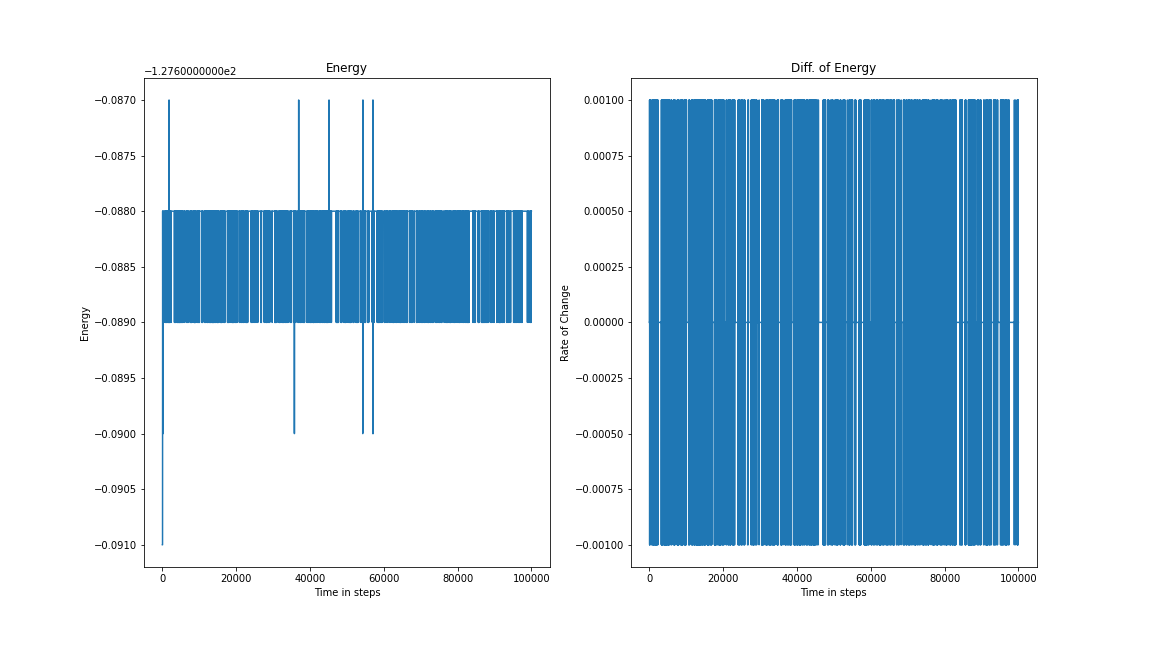
\includegraphics[scale=0.35]{Figure/plot_001.png}
	\end{center}
	\caption[Simulation]{Simulation with a time step of 0.001}
	\label{Plot001}
\end{figure}
\begin{figure}[!h]
	\begin{center}
		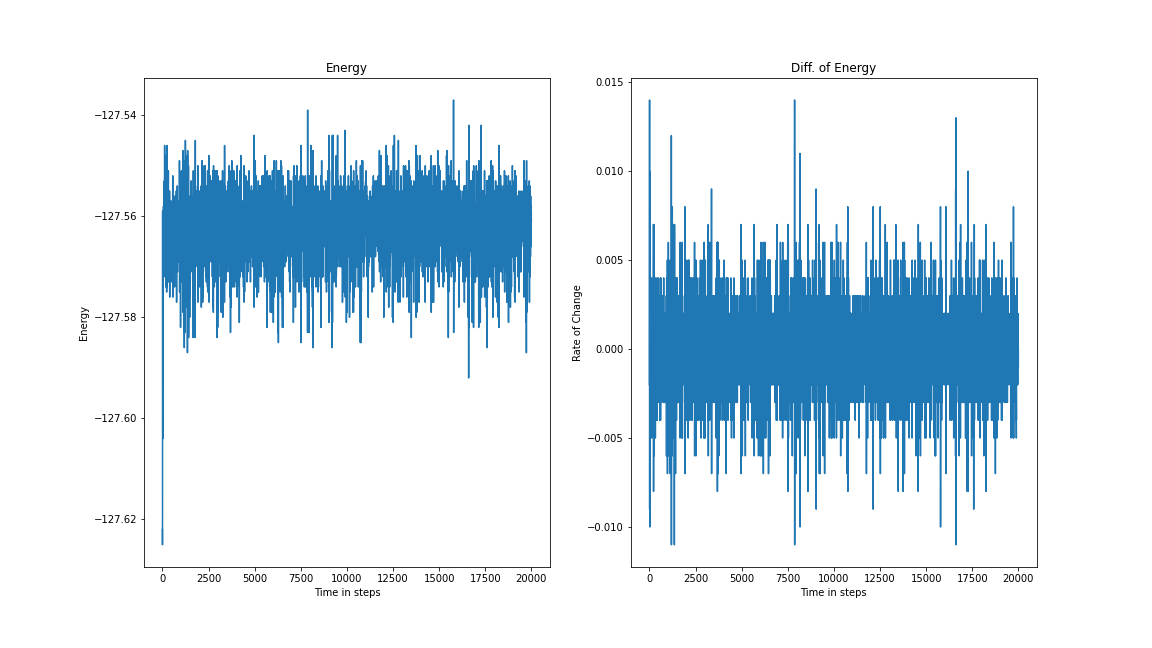
\includegraphics[scale= 0.35]{Figure/plot_005.png}
	\end{center}
	\caption[Simulation]{Simulation with a time step of 0.005}
	\label{Plot005}
\end{figure}
\begin{figure}[!h]
	\begin{center}
		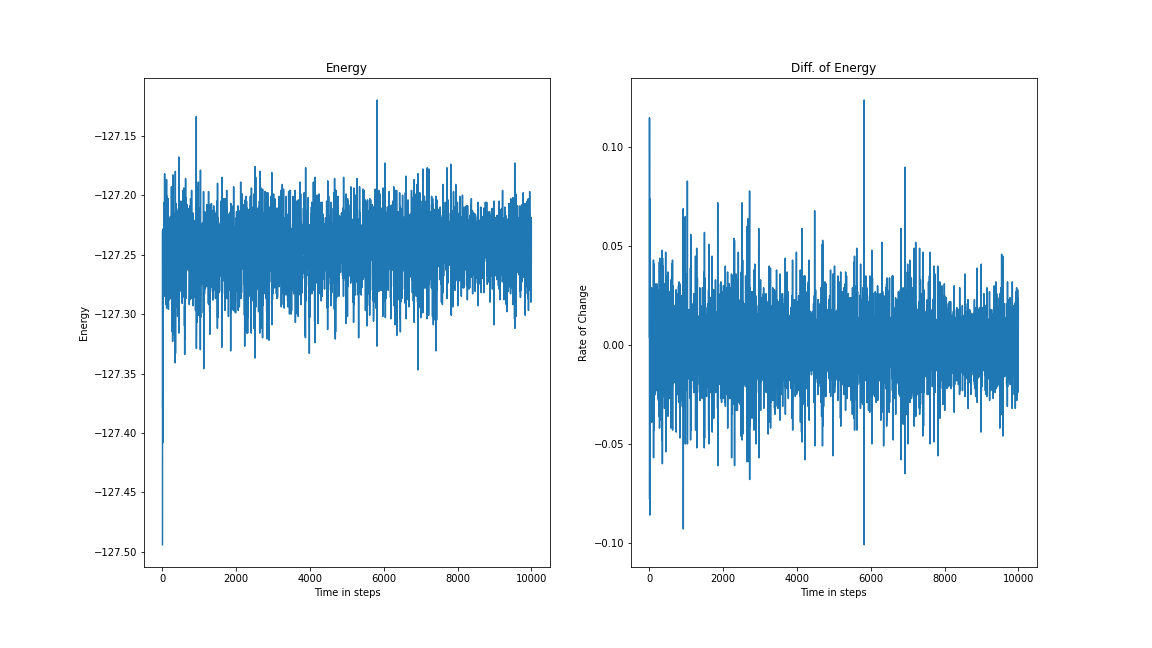
\includegraphics[scale= 0.35]{Figure/plot_01.png}
	\end{center}
	\caption[Simulation]{Simulation with a time step of 0.01}
	\label{Plot01}
\end{figure}
\begin{figure}[!h]
	\begin{center}
		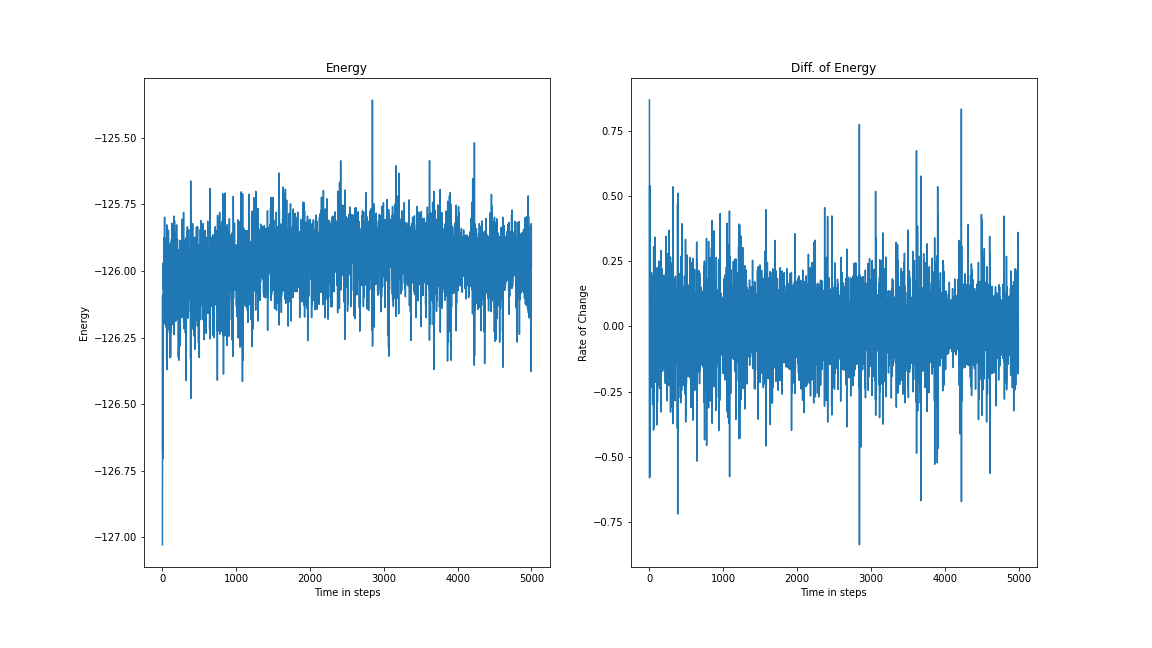
\includegraphics[scale= 0.35]{Figure/plot_02.png}
	\end{center}
	\caption[Simulation]{Simulation with a time step of 0.02 }
	\label{Plot02}
\end{figure}
\begin{figure}[!h]
	\begin{center}
		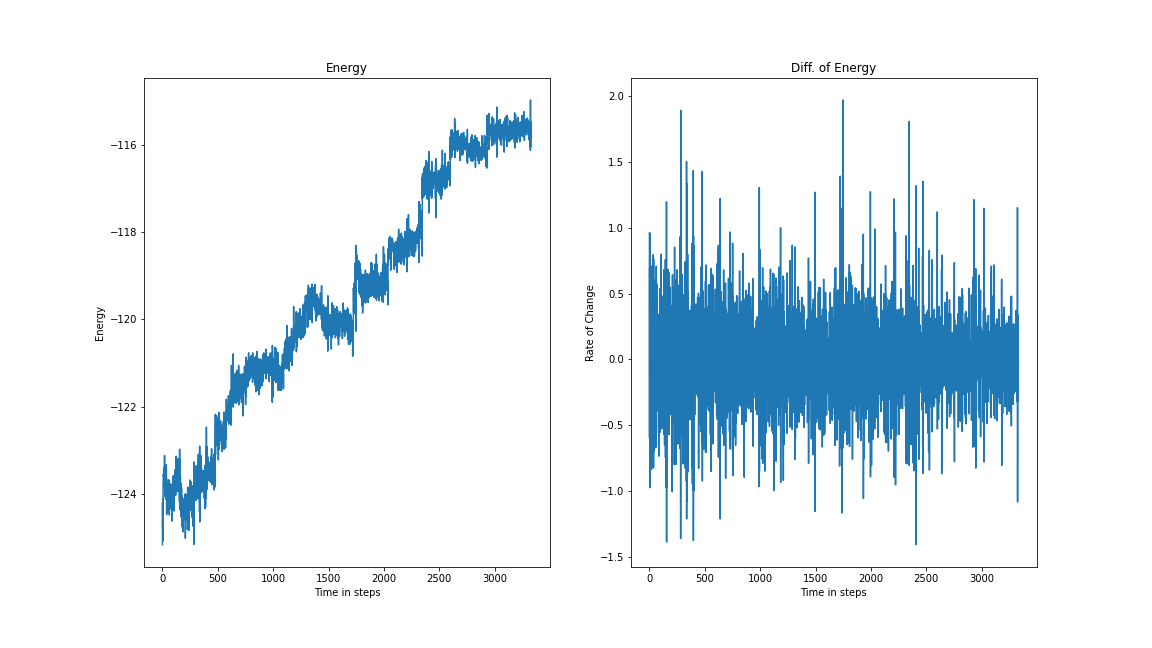
\includegraphics[scale= 0.35]{Figure/plot_03.png}
	\end{center}
	\caption[Simulation]{Simulation with a time step of 0.03 }
	\label{Plot03}
\end{figure}
\begin{figure}[!h]
	\begin{center}
		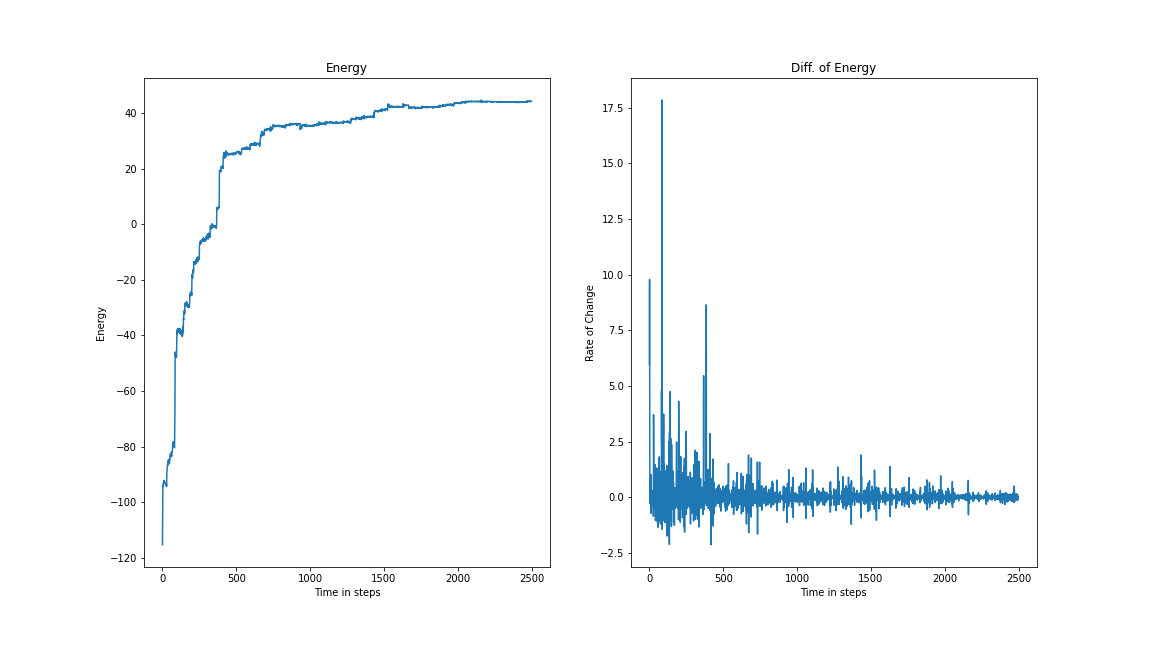
\includegraphics[scale= 0.35]{Figure/plot_04.png}
	\end{center}
	\caption[Simulation]{Simulation with a time step of 0.04 }
	\label{Plot04}
\end{figure}
%Snapshots of the simulation (5)
\section{Simulation Snapshots}
\begin{figure}[!h]
	\begin{center}
		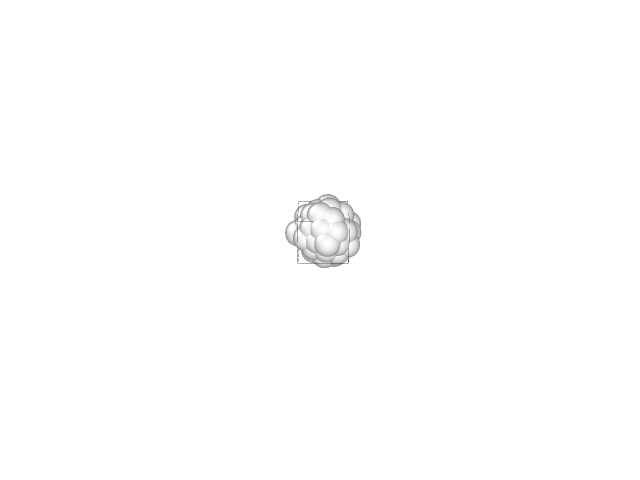
\includegraphics[scale= 1]{Figure/1Image.png}
	\end{center}
	\caption[Simulation]{Simulation }
	\label{Simulation1}
\end{figure}
\begin{figure}[!h]
	\begin{center}
		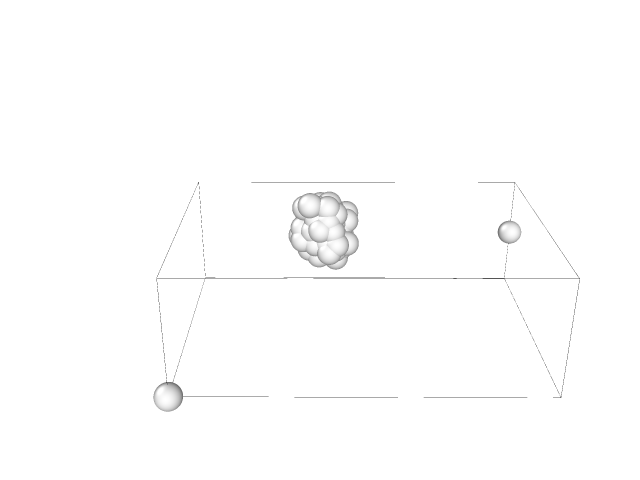
\includegraphics[scale=1]{Figure/2Image.png}
	\end{center}
	\caption[Simulation]{Simulation }
	\label{Simulation2}
\end{figure}
\begin{figure}[!h]
	\begin{center}
		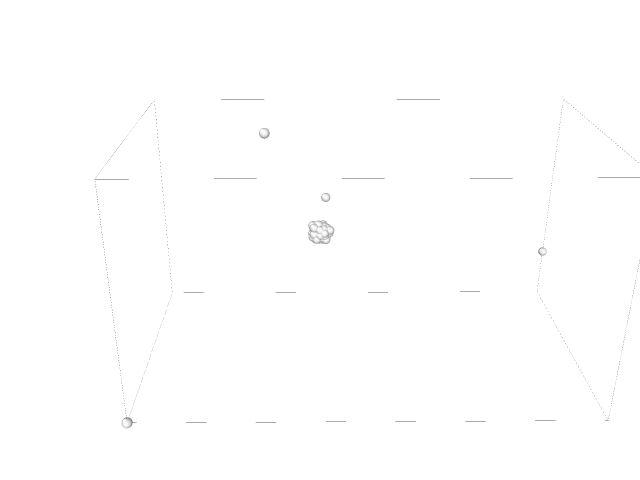
\includegraphics[scale= 1]{Figure/3Image.png}
	\end{center}
	\caption[Simulation]{Simulation }
	\label{Simulation3}
\end{figure}
\begin{figure}[!h]
	\begin{center}
		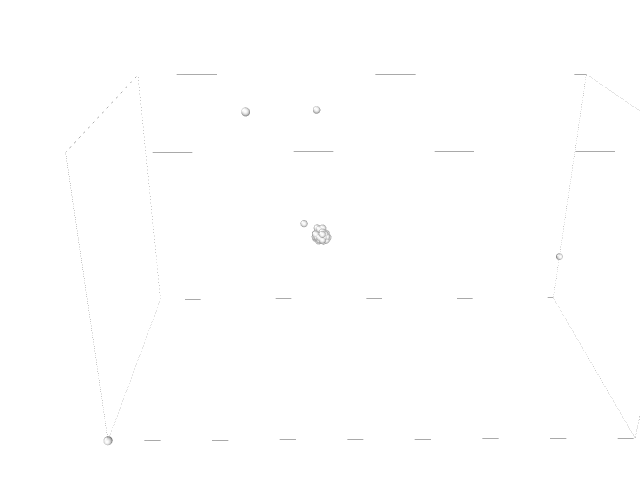
\includegraphics[scale= 1]{Figure/4Image.png}
	\end{center}
	\caption[Simulation]{Simulation }
	\label{Simulation4}
\end{figure}
\begin{figure}[!h]
	\begin{center}
		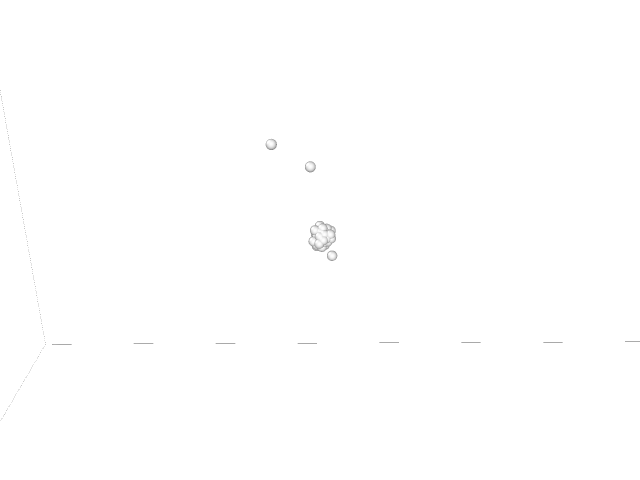
\includegraphics[scale= 1]{Figure/5Image.png}
	\end{center}
	\caption[Simulation]{Simulation }
	\label{Simulation5}
\end{figure}
%\chapter{Milestone 5}
\section{Berendsen Thermostat Teststrategy}
\begin{comment}
-basic idea is weather or not the implementation follows the exponential damping from the 2 equation for a small system with known velocities
\end{comment}
%equations
\begin{equation}
	\lambda = \sqrt{1 + \bigg(\frac{T_{0}}{T} -1\bigg)\frac{\Delta t}{\tau}}
\end{equation}

\begin{equation}
	T(t) = T_{0} + (T_{1}-T_{0})e^{-t/\tau}
\end{equation}

\section{Simulation Time}
\begin{comment}
simulation should be roughlly of complexty N2
may need too aproximate with a function 
or just argue with a single double increase
need to rerun sadly
\end{comment}
\begin{figure}[!h]
	\begin{center}
		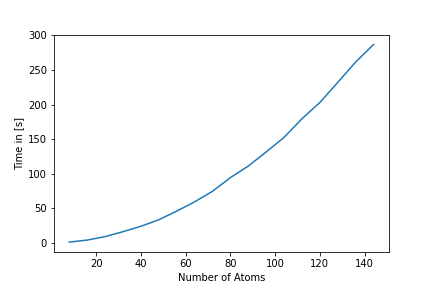
\includegraphics[scale=1]{Figure/plotAtomTimes.png}
	\end{center}
	\caption[Simulationtime]{Simulationtime from 8 to 192 Atoms }
	\label{PlotAtomTimes}
\end{figure}



%\chapter{Milestone 6}

\begin{comment}

\end{comment}
The Images are outdated!!!!
\begin{figure}[!h]
	\begin{center}
		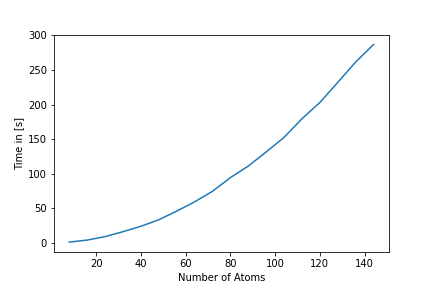
\includegraphics[scale=1]{Figure/plotAtomTimes.png}
	\end{center}
	\caption[Simulationtime without Neighborlist]{Simulationtime without Neighborlist}
	\label{PlotAtomTimesSecond}
\end{figure}
\begin{figure}[!h]
	\begin{center}
		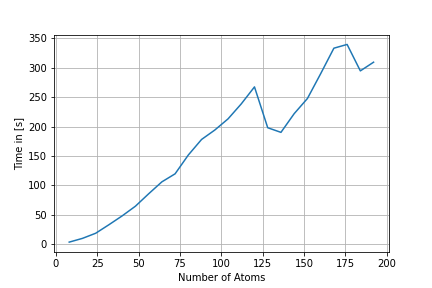
\includegraphics[scale=1]{Figure/plotAtomTimesTree.png}
	\end{center}
	\caption[Simulationtime with the old Neighborlist]{Simulationtime with the old Neighborlist}
	\label{PlotAtomTimesOldNeighbor}
\end{figure}

\begin{figure}[!h]
	\begin{center}
		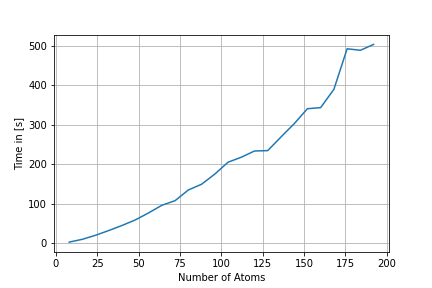
\includegraphics[scale=1]{Figure/plotAtomTimesNew.png}
	\end{center}
	\caption[Simulationtime with the new Neighborlist]{Simulationtime with the new Neighborlist  }
	\label{PlotAtomTimesCutoff}
\end{figure}
New images that are correct.
\begin{figure}[!h]
	\begin{center}
		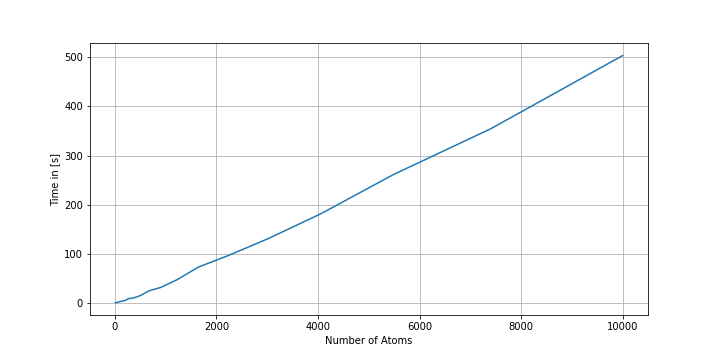
\includegraphics[scale=1.25]{Figure/plotAtomTimesMoreData.png}
	\end{center}
	\caption[Simulationtime with the new Neighborlist]{Simulationtime with the new Neighborlist  }
	\label{PlotAtomTimesCutoffNew}
\end{figure}

%% Figures for 147 Atoms 
\begin{figure}[!h] 
    \begin{center} 
        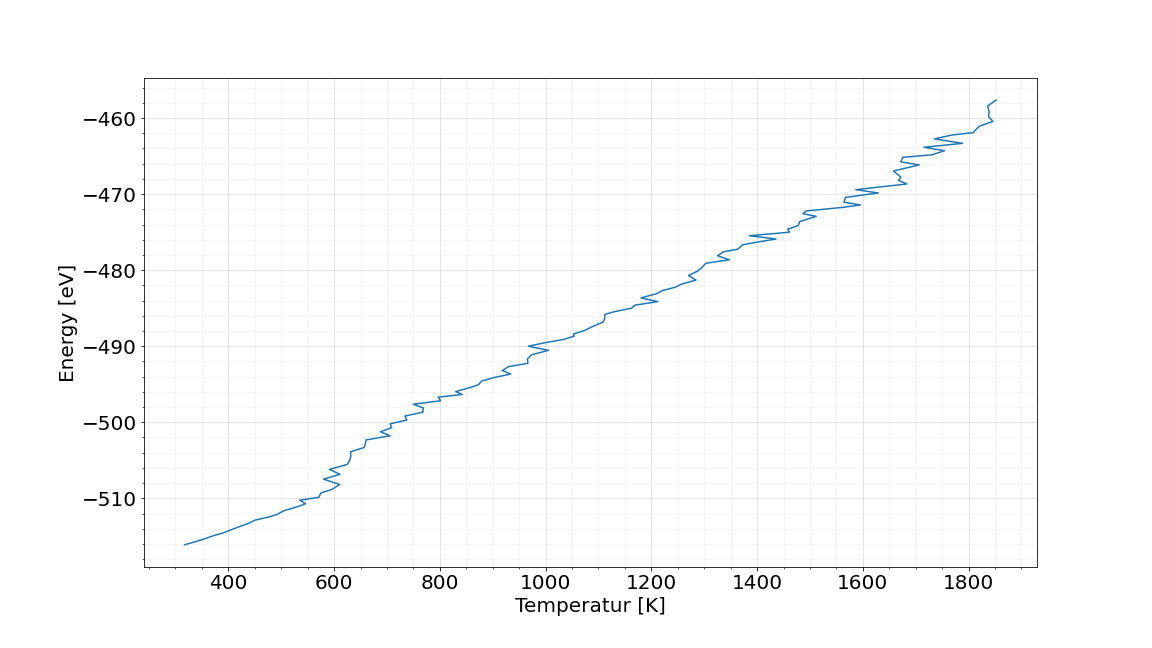
\includegraphics[scale=1.15]{/home/cm/CLionProjects/MoleDymCode/AData/Clusters/temperaturPotentialEnergyCurve3.png} 
    \end{center} 
    \caption[Gold Cluster Simulation with 147 Atoms]{Gold Cluster Simulation with 147 Atoms} 
    \label{GoldClusterSimulationTemperaturEnergy147} 
\end{figure} 
 
% Figures for 309 Atoms 
\begin{figure}[!h] 
    \begin{center} 
        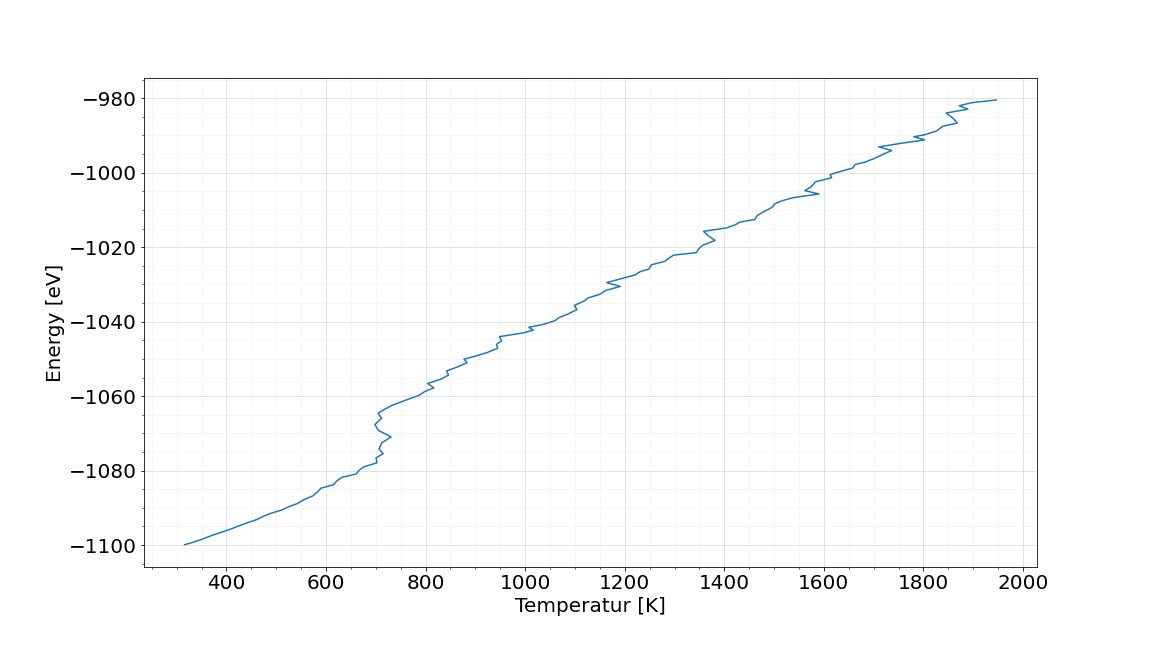
\includegraphics[scale=1.15]{/home/cm/CLionProjects/MoleDymCode/AData/Clusters/temperaturPotentialEnergyCurve4.png} 
    \end{center} 
    \caption[Gold Cluster Simulation with 309 Atoms]{Gold Cluster Simulation with 309 Atoms} 
    \label{GoldClusterSimulationTemperaturEnergy309} 
\end{figure} 
 
% Figures for 561 Atoms 
\begin{figure}[!h] 
    \begin{center} 
        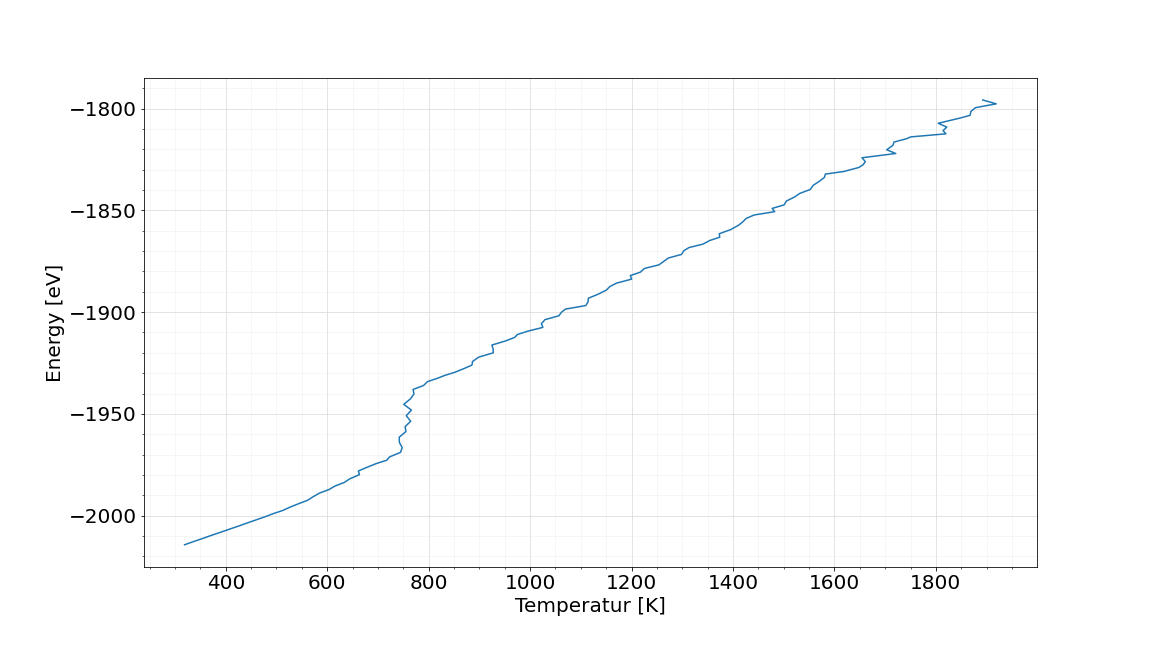
\includegraphics[scale=1.15]{/home/cm/CLionProjects/MoleDymCode/AData/Clusters/temperaturPotentialEnergyCurve5.png} 
    \end{center} 
    \caption[Gold Cluster Simulation with 561 Atoms]{Gold Cluster Simulation with 561 Atoms} 
    \label{GoldClusterSimulationTemperaturEnergy561} 
\end{figure} 
 
% Figures for 923 Atoms 
\begin{figure}[!h] 
    \begin{center} 
        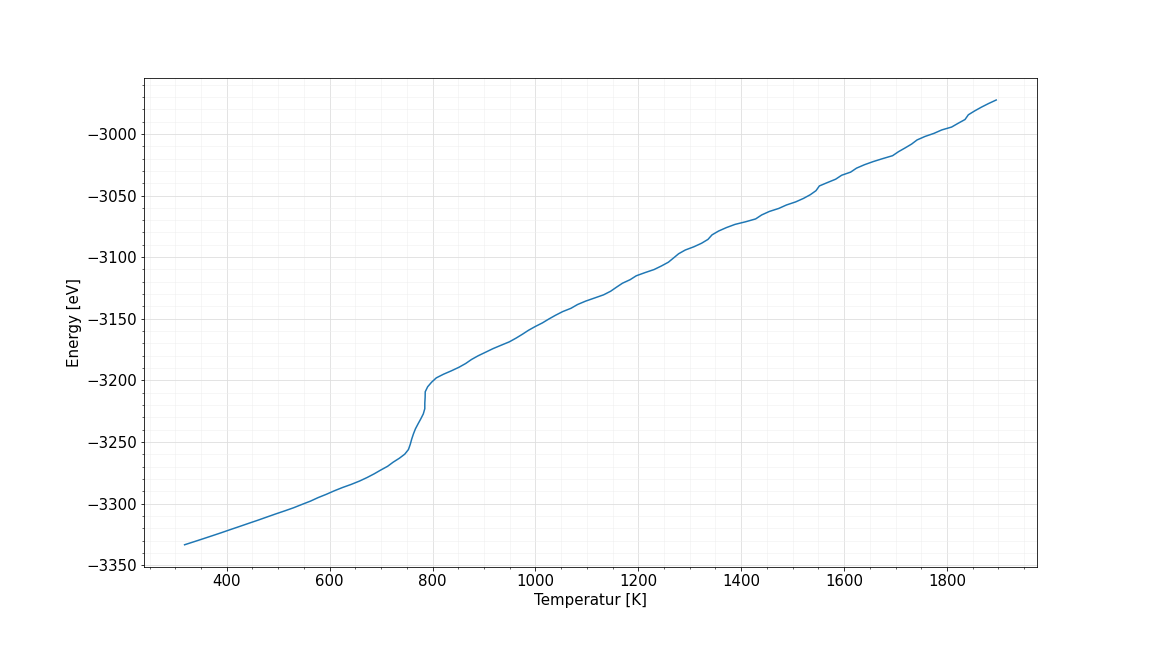
\includegraphics[scale=1.15]{/home/cm/CLionProjects/MoleDymCode/AData/Clusters/temperaturPotentialEnergyCurve6.png} 
    \end{center} 
    \caption[Gold Cluster Simulation with 923 Atoms]{Gold Cluster Simulation with 923 Atoms} 
    \label{GoldClusterSimulationTemperaturEnergy923} 
\end{figure} 
 
% Figures for 1415 Atoms 
\begin{figure}[!h] 
    \begin{center} 
        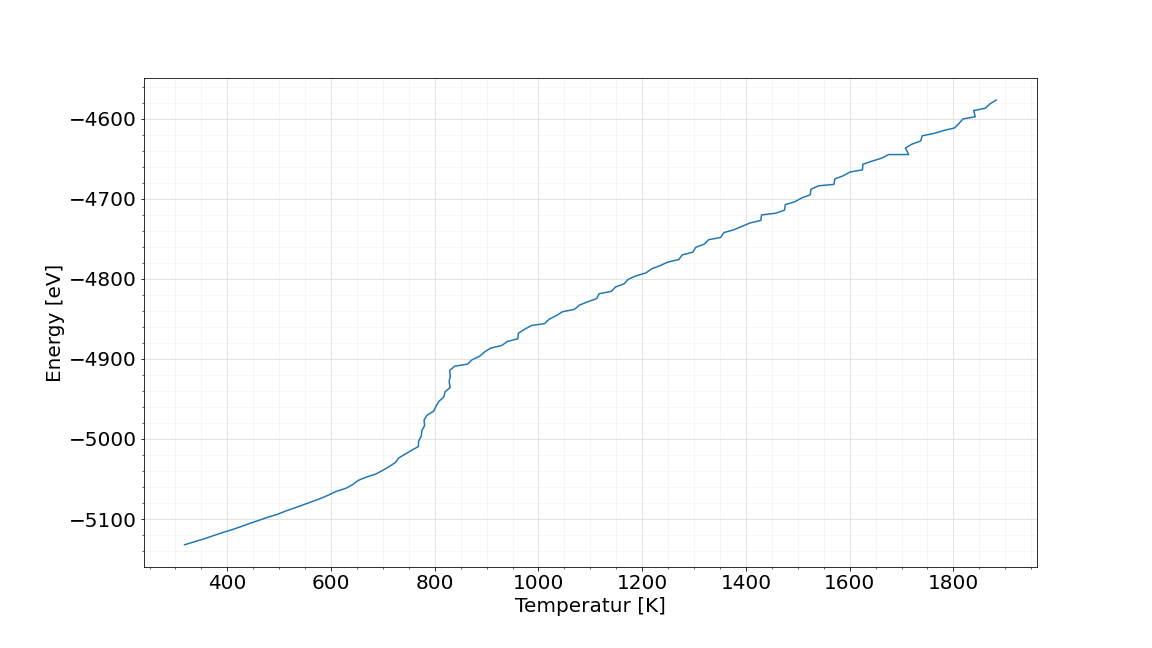
\includegraphics[scale=1.15]{/home/cm/CLionProjects/MoleDymCode/AData/Clusters/temperaturPotentialEnergyCurve7.png} 
    \end{center} 
    \caption[Gold Cluster Simulation with 1415 Atoms]{Gold Cluster Simulation with 1415 Atoms} 
    \label{GoldClusterSimulationTemperaturEnergy1415} 
\end{figure} 
 
% Figures for 2057 Atoms 
\begin{figure}[!h] 
    \begin{center} 
        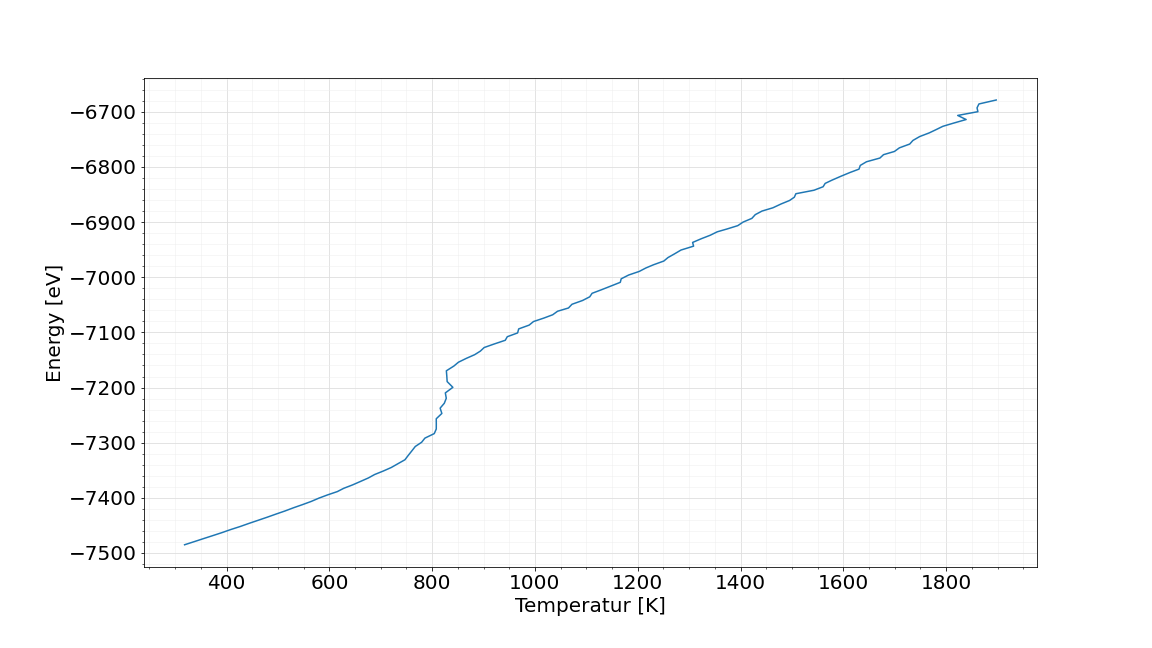
\includegraphics[scale=1.15]{/home/cm/CLionProjects/MoleDymCode/AData/Clusters/temperaturPotentialEnergyCurve8.png} 
    \end{center} 
    \caption[Gold Cluster Simulation with 2057 Atoms]{Gold Cluster Simulation with 2057 Atoms} 
    \label{GoldClusterSimulationTemperaturEnergy2057} 
\end{figure} 
 
% Figures for 2869 Atoms 
\begin{figure}[!h] 
    \begin{center} 
        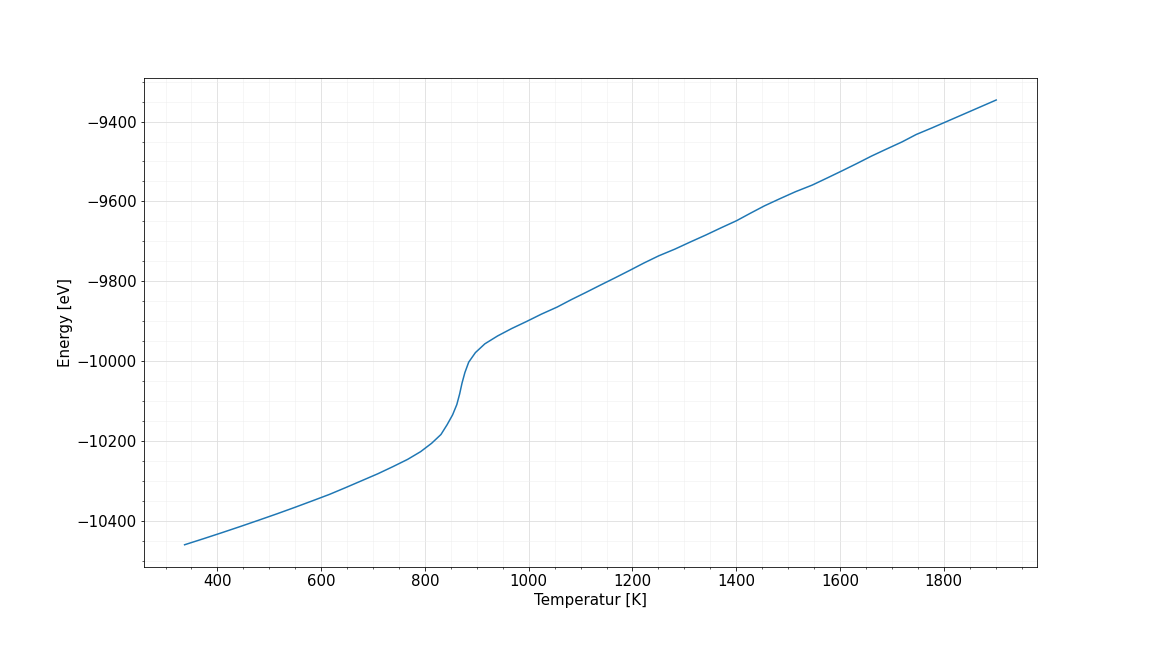
\includegraphics[scale=1.15]{/home/cm/CLionProjects/MoleDymCode/AData/Clusters/temperaturPotentialEnergyCurve9.png} 
    \end{center} 
    \caption[Gold Cluster Simulation with 2869 Atoms]{Gold Cluster Simulation with 2869 Atoms} 
    \label{GoldClusterSimulationTemperaturEnergy2869} 
\end{figure} 
 
% Figures for 3871 Atoms 
\begin{figure}[!h] 
    \begin{center} 
        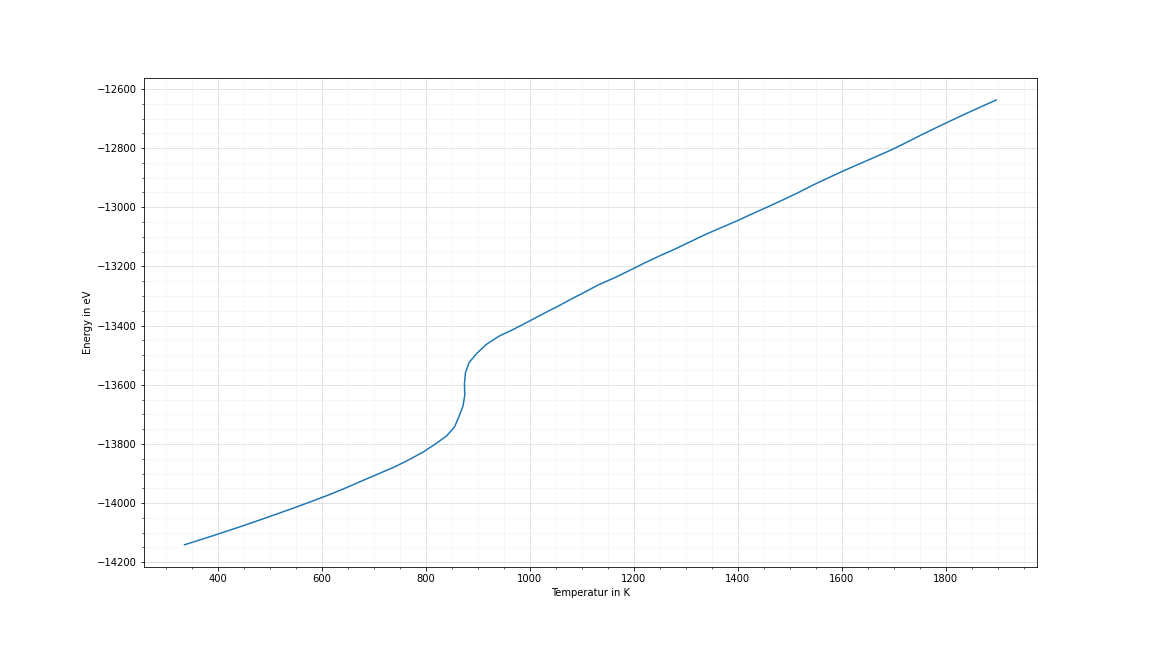
\includegraphics[scale=1.15]{/home/cm/CLionProjects/MoleDymCode/AData/Clusters/temperaturPotentialEnergyCurve10.png} 
    \end{center} 
    \caption[Gold Cluster Simulation with 3871 Atoms]{Gold Cluster Simulation with 3871 Atoms} 
    \label{GoldClusterSimulationTemperaturEnergy3871} 
\end{figure} 
 
% Figures for 5083 Atoms 
\begin{figure}[!h] 
    \begin{center} 
        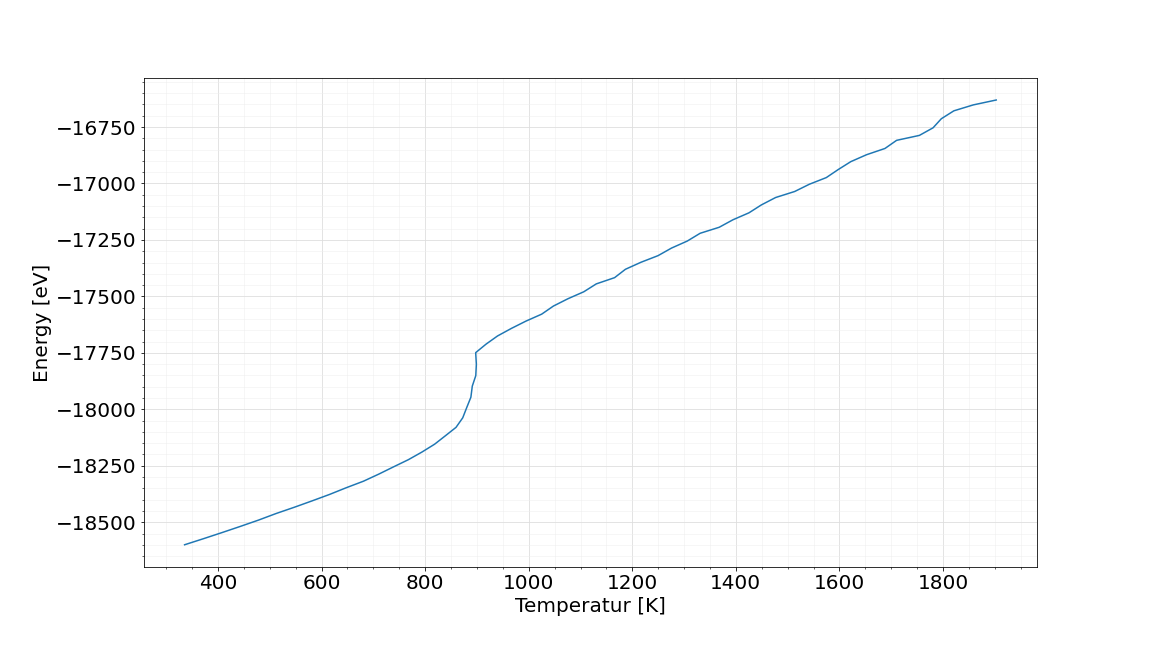
\includegraphics[scale=1.15]{/home/cm/CLionProjects/MoleDymCode/AData/Clusters/temperaturPotentialEnergyCurve11.png} 
    \end{center} 
    \caption[Gold Cluster Simulation with 5083 Atoms]{Gold Cluster Simulation with 5083 Atoms} 
    \label{GoldClusterSimulationTemperaturEnergy5083} 
\end{figure} 
 
% Figures for 6525 Atoms 
\begin{figure}[!h] 
    \begin{center} 
        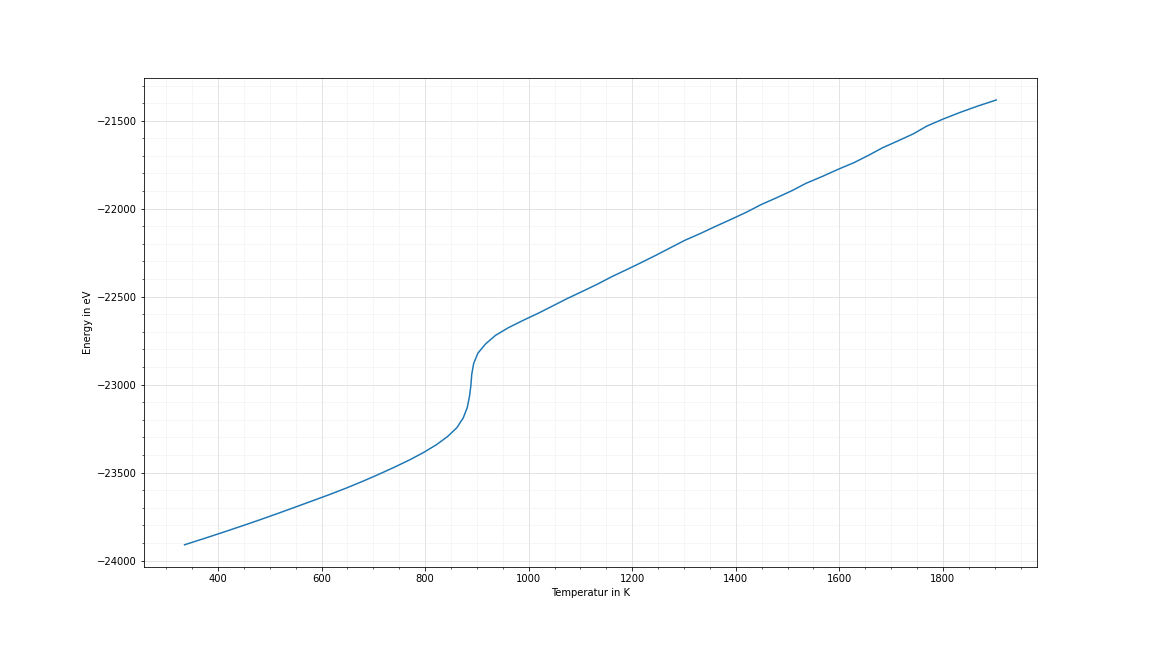
\includegraphics[scale=1.15]{/home/cm/CLionProjects/MoleDymCode/AData/Clusters/temperaturPotentialEnergyCurve12.png} 
    \end{center} 
    \caption[Gold Cluster Simulation with 6525 Atoms]{Gold Cluster Simulation with 6525 Atoms} 
    \label{GoldClusterSimulationTemperaturEnergy6525} 
\end{figure} 
 
% Figures for 8217 Atoms 
\begin{figure}[!h] 
    \begin{center} 
        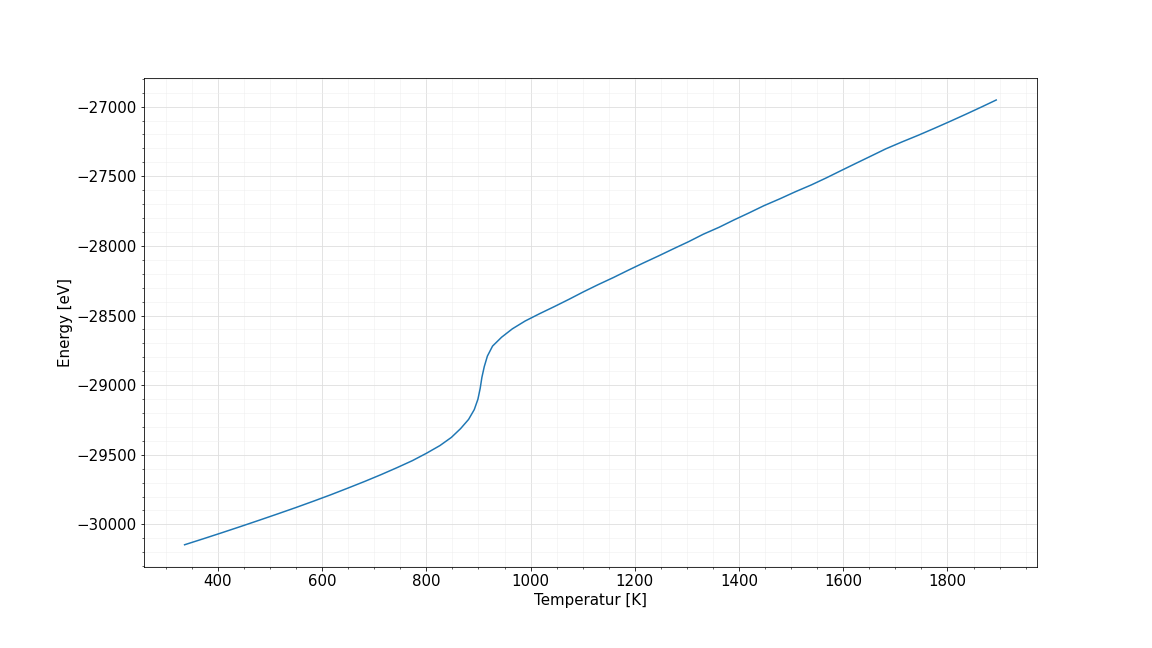
\includegraphics[scale=1.15]{/home/cm/CLionProjects/MoleDymCode/AData/Clusters/temperaturPotentialEnergyCurve13.png} 
    \end{center} 
    \caption[Gold Cluster Simulation with 8217 Atoms]{Gold Cluster Simulation with 8217 Atoms} 
    \label{GoldClusterSimulationTemperaturEnergy8217} 
\end{figure} 
 
% Figures for 10179 Atoms 
\begin{figure}[!h] 
    \begin{center} 
        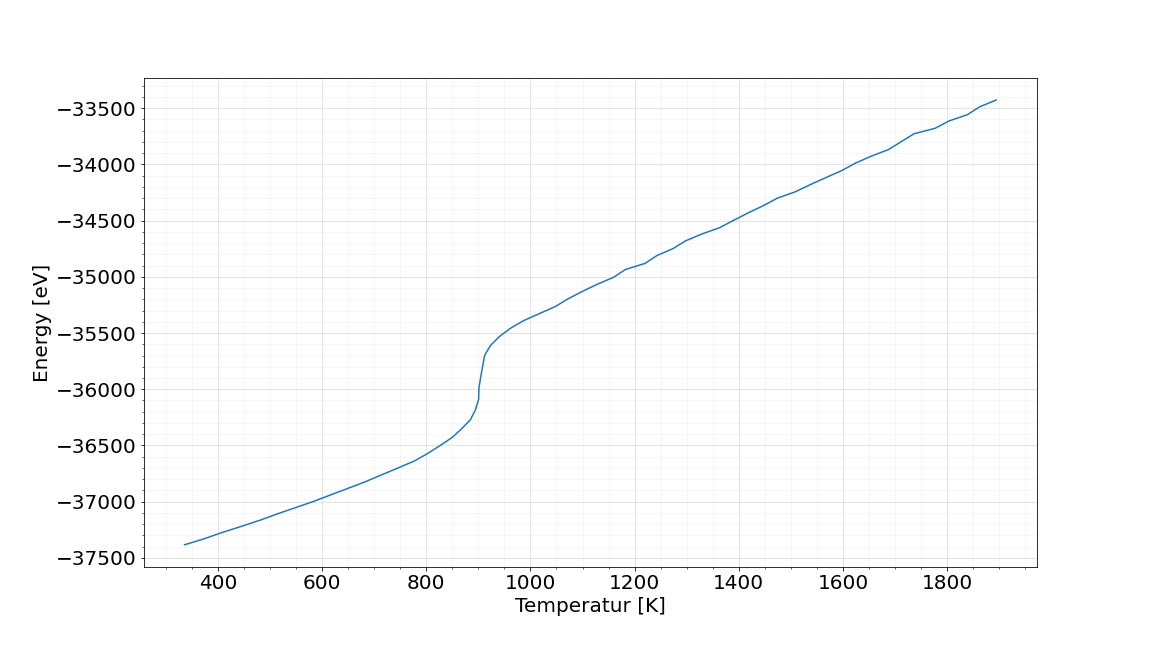
\includegraphics[scale=1.15]{/home/cm/CLionProjects/MoleDymCode/AData/Clusters/temperaturPotentialEnergyCurve14.png} 
    \end{center} 
    \caption[Gold Cluster Simulation with 10179 Atoms]{Gold Cluster Simulation with 10179 Atoms} 
    \label{GoldClusterSimulationTemperaturEnergy10179} 
\end{figure} 
 

%actual report
\tableofcontents
\listoffigures
\clearpage
\chapter{Introduction}
\begin{comment}
- atoms maybe as the first bullet point 1800 know but also the greeks knew, but was kinda forgotten again. Do i need a cite there?! nah
- with stronger computers it became possible to simulate  the atoms, but kinda computationally expensive, methods have to be developed to simplifyc  stuff
- mention like the goal of this, build an own smol simulation
- introduction to md simulation 
- weird mix between chemistry, physics and computation + a lot of programming
- written in c++ instead of the standard python stuff 
- from a developers perspective programming in python will most likely take less time, while programming in be a bit faster (and more complicated)
\end{comment}

%This is the report for the class Molecular Dynamics with C++. The goal of the course was to build a small simulation witch is an introduction to the basis of molecular dynamics. 

Since the early 1800s, it is known that all matter we can see is build from tiny particles, called atoms. With computers getting faster and faster, it is possible to simulate those particles in a computer. But as with many things there has to be made a trade-off between accuracy of the simulation and actually being able to run said simulation in a reasonable time frame, while still getting correct results. 
Developing methods for this problem, is the goal of molecular dynamics. 
\par 
In an introduction to molecular dynamics the students were tasked to write their own simulation code in C++. The methods used, the implementation itself and results gained with the code are described in this report. 
\chapter{Methods}
\begin{comment}
	0. Verlet Step
	1. Describe the Lenard Jones Potential
	2. Describe the Berendsen Thermostat
	3. Describe the Gupta 
	
\end{comment}
\begin{comment}
	Atoms are discreticed into the Postitions, Velocities and Forces 
	Second propagate the atom in the discriticed realm given constant Forces
		-> Velocity-Verlet Integration
	
	Compute Forces somehow
	-> Potentials
	LJ Potential 
	Gupta Potential
	
	Thermodynamic Effects
	Berendsen Thermostat
		->Gentle Way of resealing the Velocities
		
\end{comment}
%end general
\begin{comment}
goals of a md simulation
- determine the motion of each atom
	-> solve equation of motion 
	-> compute forces
	-> From the dirivation of the potential energy we can get the forces

- disciticed in time

\end{comment}
The goal of a molecular dynamics simulation is to determine the motion of each individual atom. For this we have to solve the equations of motion and compute the forces that affect each atom.
\begin{equation}
	\label{potentialForceEquation}
	\overrightarrow{f_{k}} = -\cfrac{\displaystyle\partial}{\displaystyle \partial \overrightarrow{r_{k}}} E_{pot}(\{\overrightarrow{r_{k}}\}) 
\end{equation}
The forces can be derived from the potential Energy as shown in \ref{potentialForceEquation} \cite[cf.][]{molDymCourse}. 


\section{Integration}
\begin{comment}
- obtain force from the previous equation
- dirivation in v. r.. from the mass
- system can be discribed just by the velocity and postion of each atom
- in the simulation the positions and velocities of the individual atoms have to be tracked and updated accordingly
- most used  is the Velocity-Verlet Algorithm
\end{comment}
From the equation \ref{potentialForceEquation} we can obtain the force at each individual atom with it's acceleration, velocity and position as shown in  \ref{potentialForceEquationForEachAtom}. 
\begin{equation}
	\label{potentialForceEquationForEachAtom}
	\overrightarrow{f_{i}} = \cfrac{\displaystyle\partial E_{pot}}{\displaystyle \partial \overrightarrow{r_{i}}} = m_{i}\overrightarrow{a_{i}} = m_{i}\overrightarrow{\dot{v_{i}}} = m_{i}\overrightarrow{\ddot{r_{i}}}
\end{equation}
It can be seen that the system can be described just by the velocities and positions of the atoms. 
In the implementation we hold these values in an container-class to ensure that they are consecutive in  memory. This speeds up the simulation. 
\par
%to porpagate
In the next step we need to somehow propagate the simulation forward in time as a static simulation would be rather boring. For updating the positions and velocities one of the most used algorithm is the Velocity-Verlet integration. 
This scheme is often split up into two steps, the prediction shown in the equations \ref{verletPrediction1} and \ref{verletPrediction2} and the correction shown in equation \ref{verletCorrection} \cite[cf. ][]{molDymCourse}. In between the two steps the force can be updated. 
%Verlet steps
\begin{equation}
	\label{verletPrediction1}
	\overrightarrow{v_{i}}(t+\Delta t/2) = 
	\overrightarrow{v_{i}}(t) + 
	\frac{\overrightarrow{f_{i}}(t)\Delta t}{2m_{i}}
\end{equation}

\begin{equation}
	\label{verletPrediction2}
	\overrightarrow{r_{i}}(t+\Delta t) = 
	\overrightarrow{r_{i}}(t) + \overrightarrow{v_{i}}(t + \Delta t/2)\Delta t
\end{equation}

\begin{equation}
	\label{verletCorrection}
	\overrightarrow{v_{i}}(t+\Delta t) = \overrightarrow{v_{i}}(t+\Delta t/2) +
	\frac{\overrightarrow{f_{i}}(t + \Delta t)\Delta t}{2m_{i}}
\end{equation}
We could now already propagate atoms forward with a constant force, so next we have to actually model the forces affecting each atom.


\section{Lenard-Jones-Potential}
\begin{comment}
- pair potential
\end{comment}
%General Formula for the dirivation
The Lenard-Jones potential is most likely one of the more famous pair potentials. The goal of them is to model the Coulomb force and the Pauli repulsion. 
\begin{equation}
	V(r) = 4\epsilon\bigg[\Big(\frac{\sigma}{r}\Big)^{12}- \Big(\frac{\sigma}{r}\Big)^{6} \bigg]
\end{equation}
As shown in \ref{potentialForceEquation} we can derive the forces from the potential Energy. Now we have to formulate the equation for each atom, this was done in \ref {potentialEquationAtoms}. We can get the force at the atom, if we get sum up the derivative of the potential energy between atom k and all the other atoms i times the normed vector between them. 
\begin{equation}
	\label{potentialEquationAtoms}
	\overrightarrow{f_{k}} = -\frac{\partial E_{pot}}{\partial  \overrightarrow{r_{k}}}=\sum_{i}^{}\frac{\partial V}{\partial r_{ik}} \hat{r_{ik}}
\end{equation}
%Formulation of the lj potential
To actually implement the equation we have to actually derive $\delta V/ \delta r_{ik}$ analytically. This could have been done by hand, but was actually just done with python. 
%Potential derivation with python
\begin{tcolorbox}[breakable, size=fbox, boxrule=1pt, pad at break*=1mm,colback=cellbackground, colframe=cellborder]
%\prompt{In}{incolor}{4}{\boxspacing}
\begin{Verbatim}[commandchars=\\\{\}]
\PY{k+kn}{import} \PY{n+nn}{sympy} \PY{k}{as} \PY{n+nn}{sp}
\PY{k+kn}{import} \PY{n+nn}{warnings}
\PY{n}{warnings}\PY{o}{.}\PY{n}{filterwarnings}\PY{p}{(}\PY{l+s+s1}{\PYZsq{}}\PY{l+s+s1}{ignore}\PY{l+s+s1}{\PYZsq{}}\PY{p}{)}
\PY{n}{sp}\PY{o}{.}\PY{n}{init\PYZus{}printing}\PY{p}{(}\PY{p}{)}
\PY{n}{eps} \PY{o}{=} \PY{n}{sp}\PY{o}{.}\PY{n}{Symbol}\PY{p}{(}\PY{l+s+s2}{\PYZdq{}}\PY{l+s+s2}{e}\PY{l+s+s2}{\PYZdq{}}\PY{p}{)}
\PY{n}{sig} \PY{o}{=} \PY{n}{sp}\PY{o}{.}\PY{n}{Symbol}\PY{p}{(}\PY{l+s+s2}{\PYZdq{}}\PY{l+s+s2}{s}\PY{l+s+s2}{\PYZdq{}}\PY{p}{)}
\PY{n}{rad} \PY{o}{=} \PY{n}{sp}\PY{o}{.}\PY{n}{Symbol}\PY{p}{(}\PY{l+s+s2}{\PYZdq{}}\PY{l+s+s2}{r}\PY{l+s+s2}{\PYZdq{}}\PY{p}{)}
\PY{n}{energyRad} \PY{o}{=} \PY{l+m+mi}{4} \PY{o}{*} \PY{n}{eps} \PY{o}{*} \PY{p}{(}\PY{p}{(}\PY{n}{sig}\PY{o}{/}\PY{n}{rad}\PY{p}{)}\PY{o}{*}\PY{o}{*}\PY{l+m+mi}{12} \PY{o}{\PYZhy{}} \PY{p}{(}\PY{n}{sig}\PY{o}{/}\PY{n}{rad}\PY{p}{)}\PY{o}{*}\PY{o}{*}\PY{l+m+mi}{6}\PY{p}{)}
\PY{n}{energyRad}\PY{o}{.}\PY{n}{diff}\PY{p}{(}\PY{n}{rad}\PY{p}{)}
	\end{Verbatim}
\end{tcolorbox}

With the codesnippet from above the derivative of the potential, shown in the next equation \ref{potentialEquationAtomsDirivative}, was obtained.
\begin{equation}
	\label{potentialEquationAtomsDirivative}
	\frac{\partial V}{\partial r} = 4 \epsilon \left(\frac{6 \sigma^{6}}{r^{7}} - \frac{12 \sigma^{12}}{r^{13}}\right)
\end{equation}
Now we can implement those last two equations. We can even optimize it by subtracting the force that affects atom k from the forces of atom i, as they have to be the same just with opposite direction and therefore sign. 

\section{Berendsen-Thermostat}

\begin{equation}
	\lambda = \sqrt{1 + \bigg(\frac{T_{0}}{T} -1\bigg)\frac{\Delta t}{\tau}}
\end{equation}

\begin{equation}
	T(t) = T_{0} + (T_{1}-T_{0})e^{-t/\tau}
\end{equation}

\section{Neighborhood-Search Algorithm}
%Not sure about that one
\begin{comment}

\end{comment}

\section{Embedded-Atom Method Potentials}
\begin{comment}
- describe Units 
- will be funny describing it in general
\end{comment}


\chapter{Implementation}
\begin{comment}	
	go about structure of the code 
	-> describe Code structure
		
	-> c++ was used to implement the code (mostly functional)
	-> key atoms container Class which holdes all the Values
	-> most functions were tested with googleTest
\end{comment}

%basic
\begin{comment}
code written in c++ most of it pretty functional, classes just used 
for the atoms container which holds the arrays 
while writing it also wrote the unittests with googletest
data aquiered form the code plotted with python
also where large simulations had to be run, called the program from the python code

\end{comment}
%TODO cite shit
The simulation code was written in C++, most of it just as functions, although the positions, velocities, etc. of the individual atoms where saved in a container-class.
While writing the functions, these were also tested with unit-tests.
Plots generation and automation for running the project were written in python.

%used software
\begin{comment}
developed in CLion which as an integrated git inviroment
Clion builds with Cmake then clang as a compiler
debugger is gdb(nicely hidden)
- additianal bibs where :
	googletest	for unittests
	eigen		for arrays 
- software used form the class itself 
- ovito for visualization
\end{comment}
The C++-code was developed in CLion, an IDE which bundles many useful features together (CMake, GDB and Git).
The python-code was written in jupyter-notebook, alternatively this could also have been done directly in CLion with a plugin. 
Additional libaries used where: googletest \cite{googletest} for the unit-tests and eigen \cite{eigen} for the arrays used for data storage in the container-class. 
Further software form the course was used for reading xyz-data and for the implementation of the Neighborhood-Search and Gupta-Potential algorithms \cite{molDymCourse}. 
To visualize the simulation the positions of the atoms at a given time where recorded and then put into OVITO Basic \cite{ovito} to be able to look at them.
\begin{comment}
--
code is structured into the milestones, so an individual milestone can be rerun in case of fuckup
parted into h and cpp files as usual
followed the structure of the milestone
\end{comment}

The code is parted into a headerfile (.h) and a codefile (.cpp). The functions where generally structured into a related header- and codefile. For example all functions regarding the Lenard-Jones-Potential can be found in an appropriately named filecombo. Furthermore a test file exists where the unit-tests can be found.
\par
The implementation itself just followed the milestones given in the course and went up till milestone seven. 
In case any mistakes happened the main of each milestone was saved into an extra file and just commented into the code again in the true main.cpp file. 
\par
For further information it would be best to just look at the code itself as it should be well commented \cite{molDymGithub}.





\chapter{Results}
\begin{comment}


\end{comment}

\section{Results from the Lenard-Jones Potential with direct Summation}
\begin{comment}

\end{comment}

% Plot of the total energy as a function of time
\begin{figure}
	\begin{center}
		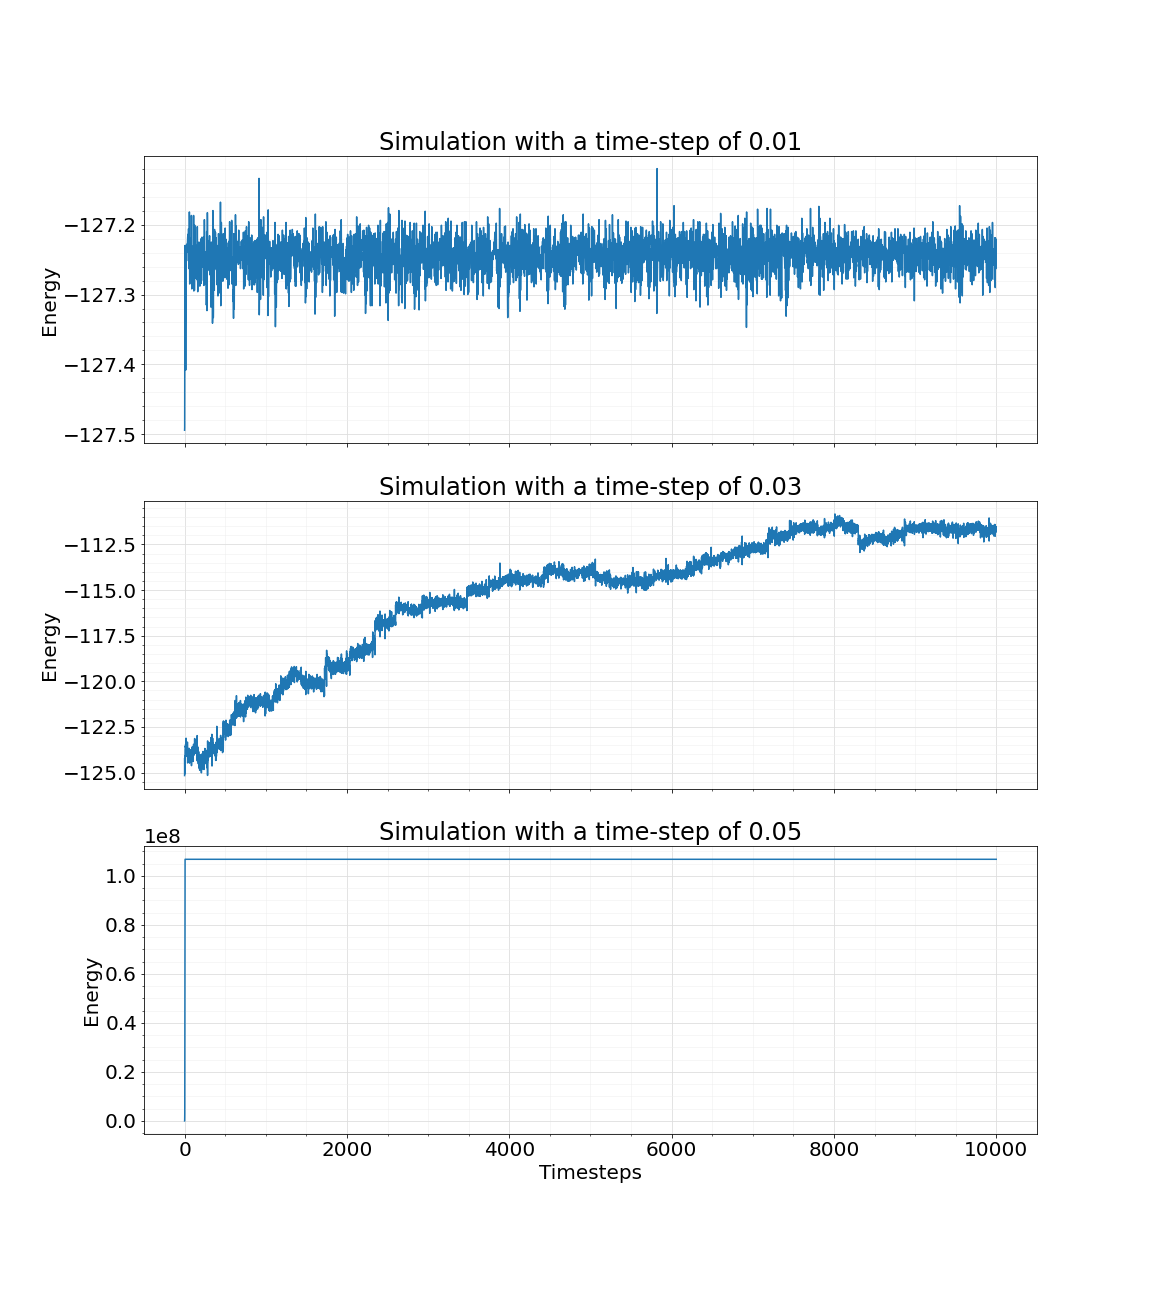
\includegraphics[scale= 1.05]{/home/cm/CLionProjects/MDCode/AData//totalEnergyDrift.png}
	\end{center}
	\caption[Simulation with different timesteps]{Simulation with different timesteps}
	\label{SimWithTimestep}
\end{figure}
The first task of the course asks to plot the total energy of the simulation for different time steps. The units were in a Lenard-Jones equivalent and not given here. As can be seen in the sequence \ref{SimWithTimestep}, with a bigger and bigger timestep the energy in the simulation goes from stable (timestep 0.01) over a drifting behavior (timestep 0.03) to being unstable (timestep 0.05). A good timestep for this simulation would be 0.01.  
\par
To visualize the simulation OVITO \cite{ovito} was used and this series of images was created.
% Simulation Snapshots
\begin{figure}
	\begin{center}
		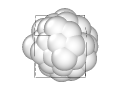
\includegraphics[scale= 0.65]{Figure/1ImageS.png}
	\end{center}
	\caption[Simulation Snapshot]{Simulation Snapshot}
	\label{SimulationSnapshot1}
\end{figure}

\begin{figure}
	\begin{center}
		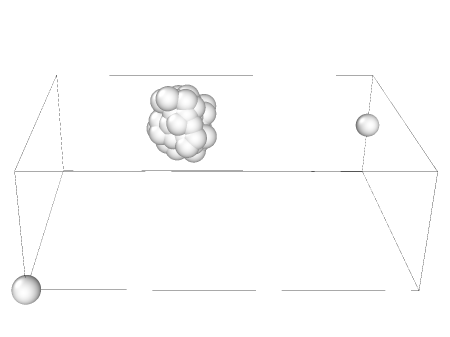
\includegraphics[scale= 0.75]{Figure/2ImageS.png}
	\end{center}
	\caption[Simulation Snapshot]{Simulation Snapshot }
	\label{SimulationSnapshot2}
\end{figure}

\begin{figure}
	\begin{center}
		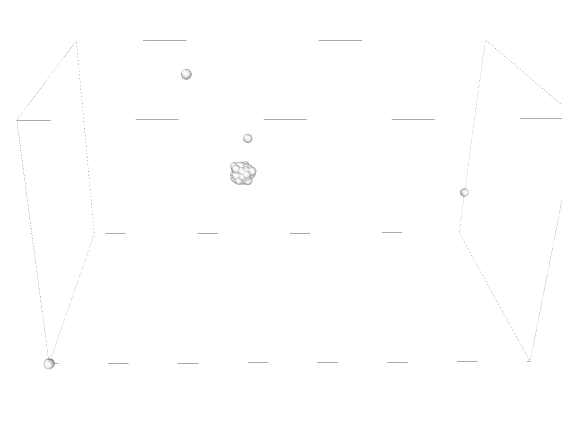
\includegraphics[scale= 0.65]{Figure/3ImageS.png}
	\end{center}
	\caption[Simulation Snapshot]{Simulation Snapshot }
	\label{SimulationSnapshot3}
\end{figure}
As it can be seen in the images \ref{SimulationSnapshot1}, \ref{SimulationSnapshot2} and \ref{SimulationSnapshot3} the Atoms are initially ordered into a blob, which was given in the course. 
Later in the simulation some of the atoms escape the initial blob and fly outward separately. 
\section{Result from the Simulation with the Berendsen Thermostat}
\begin{comment}
computational complexity 
why on2
optimization not every force is looked at individually as the force resluting form this atom is the same for the other atom but negative
\end{comment}
After incorporating the Berendsen Thermostat into the code it is interesting to look at the computational complexity of the simulation. With growing numbers of atoms the computation of should follow an order of something like O(N²). The main culprit for this is the force-computation, as each interaction with all the other atoms in the simulation has to be computed. This is also shown in the next figure as the computation time follows a quadratic function. 
\begin{figure}
	\begin{center}
		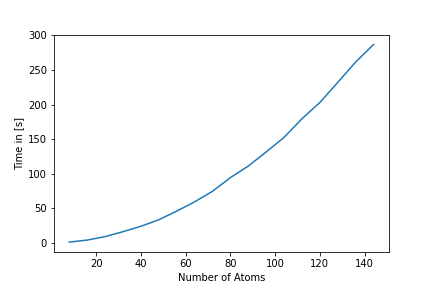
\includegraphics[scale=1]{Figure/plotAtomTimes.png}
	\end{center}
	\caption[Simulationtime with the Berendsen Thermostat from 8 to 192 Atoms]{Simulationtime with the Berendsen Thermostat from 8 to 192 Atoms }
	\label{PlotSimulationTimeBerendsenThermostat}
\end{figure}
Although all the interaction between all the atoms are computed they do not carry the same weight to the force that affects the atom. It should be rather clear that, the further apart atoms are, the smaller the force gets. After a certain distance it gets so small that it can be ignored. This leads to the idea to use neighborhood-lists that ignore the atoms outside of a certain radius, which was done in the next section.

\section{Results from the Simulation with the Neighborhood-List}
\begin{comment}

\end{comment}
After running the simulation in the previous section, it was clear that they follow a computational complexity of the order O(N²). This can be reduced to a linear order O(N) with the usage of neighborhood-lists. Only the atoms in a certain radius around the atom will be considered and a force will be added to the total force affecting the atom. This can be seen in figure \ref{PlotSimulationTimesCutoffNew} on a linear and a logarithmic scale.  
\begin{figure}
	\begin{center}
		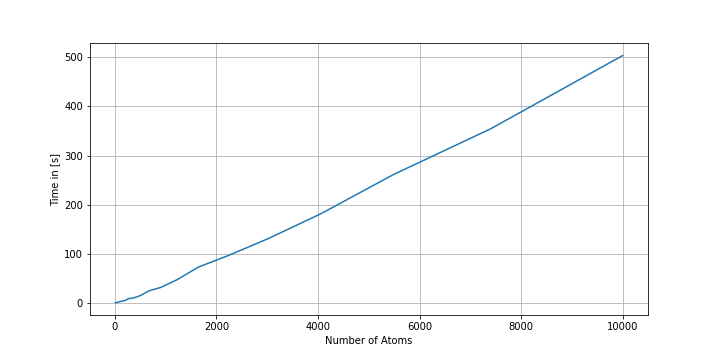
\includegraphics[scale=1.25]{Figure/plotAtomTimesMoreData.png}
	\end{center}
	\caption[Simulationtime with the Neighborhood-List]{Simulationtime with the Neighborhood-List}
	\label{PlotSimulationTimesCutoffNew}
\end{figure}

\section{Results from the Simulation with the Embedded-Atom Method Potential}
\begin{comment}
1 graph
- potential energy gets less with an increase to the clustersize
- the 

2 
Heat capacity and latent heat should converge
\end{comment}
In the next step the Embedded-Atom Method Potential was used to compute the potential energy and the forces between the atoms. A neighborhood-list was also used. With this it is possible to look at the actual physical properties of the materials in this case gold. In the figure \ref{GoldClusterSimulationTemperaturEnergy4In1} energy and temperature for different cluster sizes are plotted. It is possible to extract the melting point, the heat-capacity and the latent-heat from this diagram. This can be seen in the next figure \ref{GoldClusterSimulationVsClustersize} in relation to the size of the atom-cluster. All data in this figure has been read by hand so it has to be taken with a grain of salt. 

\par 
The first interesting property is the melting point of the cluster, which can be seen in the different curvature in the graphs in figure \ref{GoldClusterSimulationTemperaturEnergy4In1} (for the red graph at 900K for example). The melting point increases as the clusters get bigger, but still is not near it's macroscopic equivalent of 1337 K. 

\par
It can also be seen that the potential energy of the median atom sinks with bigger clustersizes. To explain this, the ratio of surface to volume of the cluster and the fact that atoms at the border of the cluster need to have a higher energy, have to be considered. With increased clustersizes a smaller percentage of atoms is at the edge and increases the total energy of the cluster. 
The slope of the curvature at the melting point also increases with bigger clustersizes. In a big physical system this actually would be straight line where the melting point is and the simulated system seems to converge to that. 

\begin{figure}
	\begin{center} 
		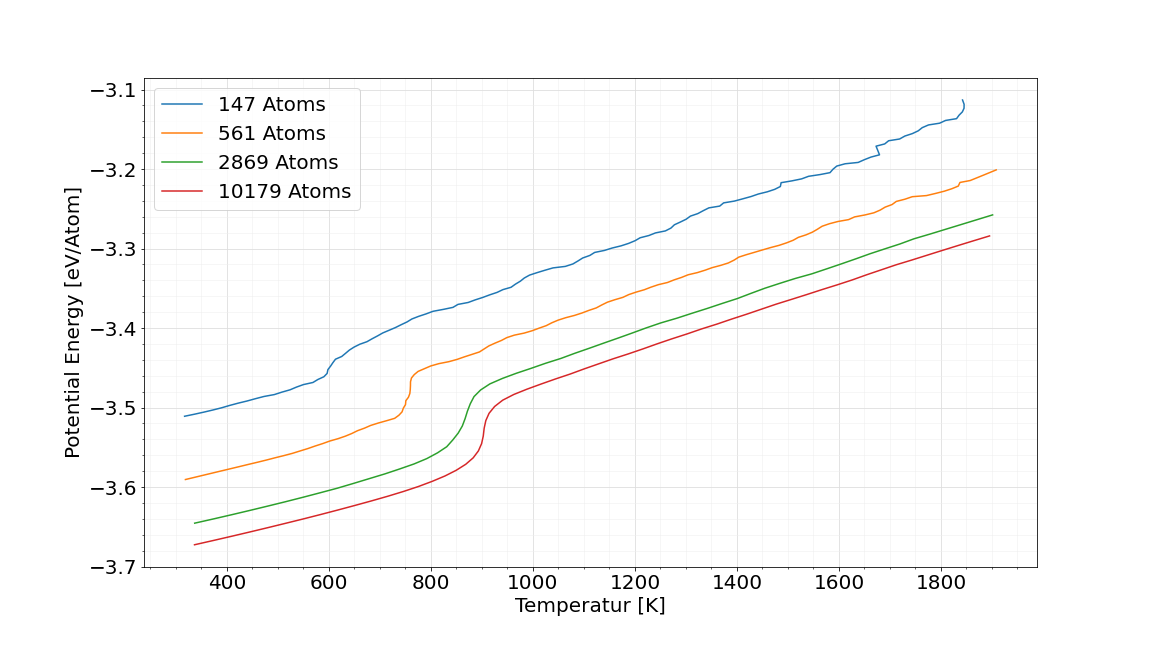
\includegraphics[scale=1.15]{/home/cm/CLionProjects/MDCode/AData/Clusters/temperaturPotentialEnergyCurveMoreInOne.png} 
	\end{center} 
	\caption[Gold Cluster Simulation]{Gold Cluster Simulation} 
	\label{GoldClusterSimulationTemperaturEnergy4In1} 
\end{figure} 

In the next figure \ref{GoldClusterSimulationVsClustersize} in the diagrams which plot the heat capacity and the latent heat, it can be seen that both seem to converge. The melting point on the other hand still seems to increase as it is still away from it's true melting point.

\begin{figure}
	\begin{center} 
		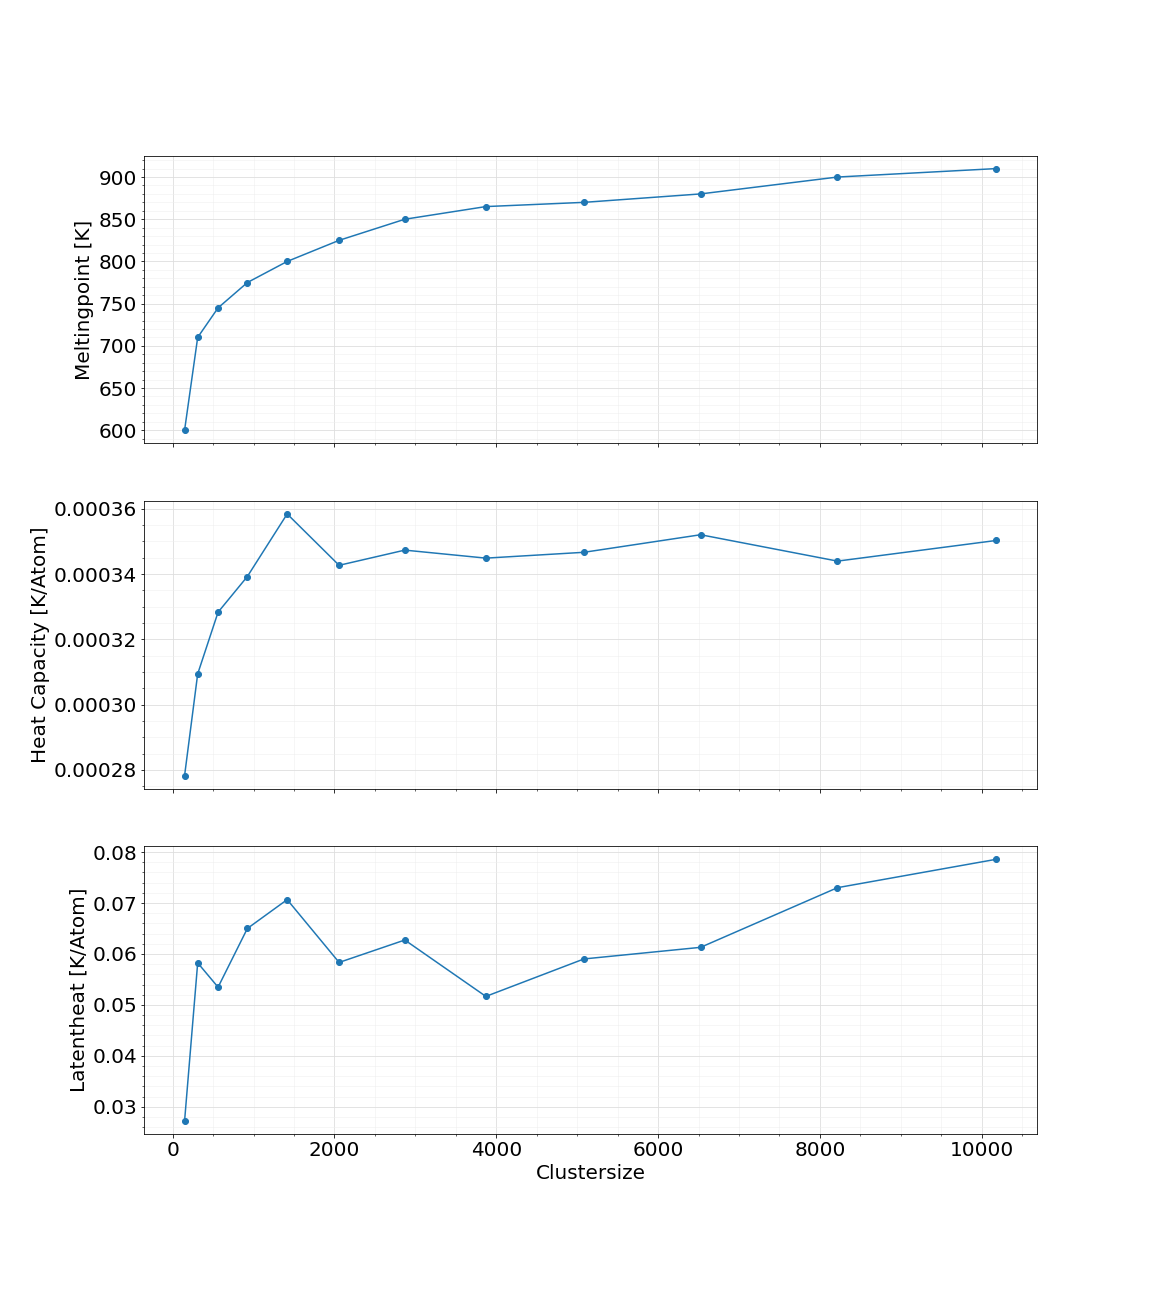
\includegraphics[scale=1.15]{/home/cm/CLionProjects/MDCode/AData/Clusters/VsClusterSizeAll.png} 
	\end{center} 
	\caption[Melting Point, Heat Capacity and Latent Heat vs Clustersize]{Melting Point, Heat Capacity and Latent Heat vs Clustersize} 
	\label{GoldClusterSimulationVsClustersize} 
\end{figure} 

\chapter{Conclusion}
\begin{comment}
- give look at stuff i did and did not
- mention all the other cool stuff, parralell hardware memes domain decompasition looking at other mechanical parameters ia stress
- should be written nice if i wanna work with those guys
\end{comment}
% %bib 

\printbibliography
\cleardoublepage

\cleardoublepage
 
\end{document}
